\documentclass[]{article}
\usepackage{lipsum}
\usepackage{float}
\usepackage{amsmath}
\usepackage{amssymb}
\usepackage[a4paper,bindingoffset=0.2in,%
left=1in,right=1in,top=1in,bottom=1in,%
footskip=.25in]{geometry}
\usepackage{graphicx}
\usepackage{caption}
\usepackage{subcaption}
\usepackage{braket}
\usepackage{mhchem}
\usepackage[english]{babel}
\usepackage[utf8]{inputenc}
\usepackage[style = numeric-comp, bibstyle = science, sorting = none]{biblatex}
\addbibresource{Graphene.bib}
%Includes "References" in the table of contents
\usepackage[nottoc]{tocbibind}
\usepackage{hyperref}
\hypersetup{
	colorlinks = true,
%	citecolor=black,
%	filecolor=black,
%	linkcolor=green,
%	urlcolor=black,
	breaklinks,
	linktocpage
}
\usepackage[hyphenbreaks]{breakurl}
\usepackage{url}
\def\UrlBreaks{\do/}
\setlength\parindent{0cm}
	
%References using Citatonsy

%opening
\title{Graphene Quantum Optics}
\author{Ruchir Tullu}
\date{August 2020}


\begin{document}

\begin{titlepage}
	    \begin{center}
		\vspace*{1cm}
		
		\Huge
		\textbf{Investigating Optical Defects in Graphene for Quantum Network Applications}
		
	%	\vspace{0.5cm}
	%	\LARGE
	%	Thesis Subtitle
		
		\vspace{0.5cm}	%1.5
		\large
		\textbf{Ruchir Tullu}
		
		\vfill
		
		\large
		A research document prepared for the \\
		Simon Group at the University of Calgary
		
		\vspace{0.8cm}
		
		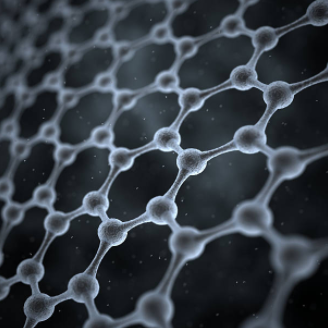
\includegraphics[width=0.6\textwidth]{graphene.PNG}
		
		\vfill
		
		\Large
		Institute for Quantum Science and Technology\\
		University of Calgary\\
		Canada\\
		October 2020
		
	\end{center}
\end{titlepage}
\thispagestyle{plain}
\begin{center}
    \Large
    \textbf{Investigating Optical Defects in Graphene for Quantum Network Applications}
    
    %\vspace{0.4cm}
   % \large
   % Thesis Subtitle
    
    \vspace{0.4cm}
    \large
    \textbf{Ruchir Tullu}
    
    \vspace{0.9cm}
    \textbf{Abstract}
\end{center}
In this report we discuss the effects of dissipation dilution and strain engineering as relevant
to cavity optomechanics. We begin by discussing basic optomechanics theory, then review strain
engineering and dissipation dilution. Finally, we present some numerical simulation results done
in COMSOL Multiphysics to simulate the effects of dissipation dilution and strain engineering
in mechanical resonators. We also present some alternative resonator designs and their advantages and
disadvantages over the tapered PnC design. The results obtained in COMSOL show signs of
approaching the mode shape required, however more work is required for this to accurately represent
the mode shape obtained by Ghadimi et al. for the tapered PnC nanobeams.


\newpage
\tableofcontents
\newpage


\section{Introduction}
Graphene is a two-dimensional honeycomb lattice of carbon atoms. Graphene is known for its exceptional electronic and structural properties \cite{The_Electronic_Properties_of_Graphene, Properties_of_graphene:_a_theoretical_perspective}. Up until the last decade, it was believed that isolated graphene sheets could not exist due to thermal and other excitations \cite{Lecture5}. However in 2004, Geim et al. demonstrated that isolated graphene sheets exist, and could be observed using simple spectroscopy \cite{Graphene_Scotch_Tape}. Since then, graphene has been an active area of research, with potential applications in quantum networks, semiconductor physics, condensed matter physics, chemistry, and electrical engineering \cite{Properties_of_graphene:_a_theoretical_perspective}. 
\newline

In this report, we will discuss the electronic structure of graphene, and how its properties can be understood in terms of the tight binding model. Then, we will look at several different promising single photon quantum emitter candidates, including graphene, hexagonal boron nitride (hBN), and several transition metal dichalcogenides (TMDCs). Finally, we will look at some DFT simulations performed using \textit{Quantum Espresso} \cite{quantum_espresso} which look at the bandgap and density of states of a few promising candidates for single photon quantum emitters. 



\section{Electronic \& Crystal Structure}

Graphene is a 2D hexagonal (honeycomb) lattice of carbon atoms. Carbon has an atomic configuration of 1$s^2$2$s^2$2$p^2$, meaning that there are four valence electrons per carbon atom. Each carbon atom in the lattice is bonded to three other carbon atoms, thereby resulting in a $sp^2$ hybridization of orbitals. These hybrid orbitals are formed between one s-orbital and two p-orbitals in a trigonal planar structure \cite{The_Electronic_Properties_of_Graphene}. The in-plane bonding between carbon atoms leads to the formation of $\sigma$ bonds, which are the result of the $sp^2$ hybridization between the 2$s$, 2$p_x$, and 2$p_y$ orbitals for three of the four valence electrons. In contrast,  the out-of-plane perpendicular 2$p_z$ orbitals, each containing one valence electron, from adjacent carbon atoms form $\pi$ bands \cite{Properties_of_graphene:_a_theoretical_perspective}. We will investigate the properties of monolayer, bilayer, and stacked graphene in the following sections.

\subsection{Monolayer Graphene}
Graphene's honeycomb lattice is an arrangement of two interlocking triangular lattices, $A$ and $B$ (see Figure \ref{fig: Graphene lattice and FBZ} below). The overall lattice is not a Bravais lattice, however we can consider it as a triangular lattice with a basis of two atoms per unit cell \cite{The_Electronic_Properties_of_Graphene}. The real-space lattice translation vectors can be written as:

\begin{equation}
	\mathbf{a_1} = \frac{a}{2}(3, \sqrt{3}), \ \ \ \ \mathbf{a_1} = \frac{a}{2}(3, -\sqrt{3})
\end{equation}

Here, $a \approx$ 1.42 $\dot{A}$ is the inter-carbon distance. The reciprocal lattice vectors can then be written as:

\begin{equation}
	\mathbf{b_1} = \frac{2\pi}{3a}(1, \sqrt{3}), \ \ \ \ \mathbf{b_1} = \frac{2\pi}{3a}(1, -\sqrt{3})
\end{equation}

Note that these vectors satisfy the orthogonality relation:

\begin{equation}
	\mathbf{a_{i} \cdot b{_{j}}} = 2\pi \delta_{ij}
\end{equation}

We can then find the First Brillouin Zone (FBZ), formed by considering the area enclosed between the the planes that are perpendicular bisectors of the reciprocal lattice vectors extending from the origin. \\

\begin{figure}[htb]
	\centering
	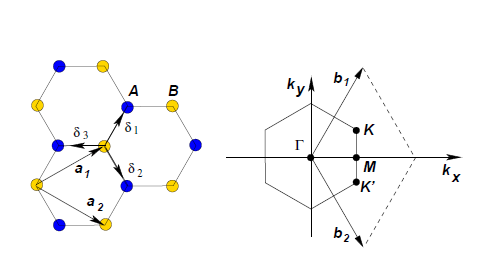
\includegraphics[scale = 0.75]{graphene_lattice.PNG}
	\caption{Lattice structure and FBZ of graphene. The left picture shows the overlapping triangular lattices to create the hexagonal/honeycomb lattice of graphene.Here, $a_1, a_2$ are the lattice unit vectors,and $\delta_i$, i = 1, 2, 3 are the nearest neighbor vectors. The right figure shows the FBZ for the corresponding honeycomb lattice. The high symmetry points $\Gamma$ and $M$ are shown along with the reciprocal lattice vectors $b_1, b_2$. The points denoted $K$ and $K'$ are known as the Dirac points. This figure is from  Castro et al. \cite{The_Electronic_Properties_of_Graphene}}
	\label{fig: Graphene lattice and FBZ}
\end{figure}

The six points at the corner of the FBZ fall into one of two groups which are equivalent due to symmetry considerations. These are labeled $K$ and $K'$ in Figure \ref{fig: Graphene lattice and FBZ}. The coordinates of these points in reciprocal lattice space are given as:

\begin{equation}\label{eq: Dirac Points}
\mathbf{K} = \frac{2\pi}{3a}(1, 1/\sqrt{3}), \ \ \ \ \mathbf{K'} = \frac{2\pi}{3a}(1, -1/\sqrt{3})
\end{equation}

It is important to note that these two points are not connected by a reciprocal lattice vector, thus they are independent values of k \cite{Lecture5}. The nearest neighbor vectors $\delta_i$ have positions in real space as given in equation \ref{eq: nearest_neighbors}:

\begin{equation}\label{eq: nearest_neighbors}
	\mathbf{\delta_1} = \frac{a}{2}(1, \sqrt{3}), \ \ \ \ \ \ \ \ \ \ \ \ \ \ \ \ \mathbf{\delta_2} = \frac{a}{2}(1, -\sqrt{3}), \ \ \ \  \ \ \ \ \ \ \ \ \ \ \ \ \mathbf{\delta_3} = -a(1, 0)
\end{equation}


The second-nearest neighbors have positions in real space as follows:

\begin{equation}
\mathbf{\delta^{'}_1} = \pm a_1, \ \ \ \ \ \ \ \ \ \ \ \ \ \ \ \ \mathbf{\delta^{'}_2} = \pm a_2, \ \ \ \  \ \ \ \ \ \ \ \ \ \ \ \ \mathbf{\delta^{'}_3} = \pm (a_2 - a_1)
\end{equation}

The tight-binding model (see section \ref{sec: Tight Bonding} for more information) Hamiltonian, considering electrons hopping in both nearest and next-nearest neighbor atoms is:

\begin{align}
	H  = -t &\sum_{<i,j>, \sigma} \bigg( a_{\sigma, i}^\dagger b_{\sigma, j} + h.c. \bigg )\\
	-t^{'} &\sum_{<<i,j>>, \sigma} \bigg( a_{\sigma, i}^\dagger a_{\sigma, j}  + b_{\sigma, i}^\dagger b_{\sigma, j} + h.c. \bigg )
\end{align}

The factors of $\hbar$ have been suppressed. Here, $a_{\sigma, i}$ annihilates an electron with spin $\sigma$ at site $R_i$ on sublattice A \cite{The_Electronic_Properties_of_Graphene}; similarly, $a_{\sigma, i}^\dagger$ is the creation operator. A similar definition is applicable to sublattice B as well. Here, $t \approx 2.8 eV$ is the nearest neighbor hopping energy (hopping between different sublattices), and $t^{'}$ is the next nearest neighbor hopping energy\footnotemark (hopping in the same sublattice) \cite{The_Electronic_Properties_of_Graphene}. The energy bands resulting from this Hamiltonian are of the form:

\footnotetext{The value of $t^{'}$ obtained from ab-initio calculations ranges from $0.02t \leq t^{'} \leq 0.2t$ \cite{The_Electronic_Properties_of_Graphene}.}

\begin{align}\label{eq:Full_Band_Equation}
	&E_{\pm}(k) = \pm t\sqrt{3+f(k)} -t^{'}f(k) \\
	&f(k) = 2\cos(\sqrt{3}k_y a) + 4\cos(\frac{\sqrt{3}}{2}k_y a)\cos(\frac{3}{2}k_x a)
\end{align}

The upper ($\pi$) and lower ($\pi^*$) bands have energies of $E_+$ and $E_-$, respectively. The energy spectrum is thus symmetric if $t^{'} = 0$; this case is plotted in Figure \ref{fig: Graphene Band}.
\newline

In the nearest neighbor approximation this reduces to \cite{Properties_of_graphene:_a_theoretical_perspective}:

\begin{equation}
	E_{\pm}(k_x, k_y) = \pm\gamma_0 \bigg [ 1 + 4\cos \frac{\sqrt{3}k_x a}{2}\cos \frac{k_y a}{2} + 4\cos^2 \frac{k_y a}{2} \bigg ]^{1/2}
\end{equation}

Here, $\gamma_0$ is the transfer integral energy between nearest neighbors \cite{Properties_of_graphene:_a_theoretical_perspective}. 
\newline

As can be seen from Figure \ref{fig: Graphene Band}, the $\pi$ and $\pi^*$ bands are degenerate near the Dirac points as given by equation \ref{eq: Dirac Points}. Taylor expanding the energy dispersion relation in equation \ref{eq:Full_Band_Equation} near these points\footnotemark leads to the following dispersion relation:

\begin{equation}\label{eq: Linear_Dispersion_Graphene}
	E_{\pm}(q) \approx \pm \frac{3ta}{2} |q| + \mathcal{O}((q/K)^2) = \pm v_F |q| + \mathcal{O}((q/K)^2)
\end{equation}

\footnotetext{We write the electron wave vector as $k = K + q$, with $|q| << |K|$ \cite{The_Electronic_Properties_of_Graphene}}

Here, $v_F$ represents the Fermi velocity, with $v_F \approx 10^6 \ m/s$ \cite{Wallace_1947_Band_Theory_Graphite}. Note the difference of this dispersion relation from that of a free particle with $E(q) = q^2/2m$; in the free particle case, the velocity is dependent on the energy and momentum as $v = k/m = \sqrt{2E/m}$ \cite{The_Electronic_Properties_of_Graphene}. The Fermi velocity in (\ref{eq: Linear_Dispersion_Graphene}) does not depend on the momentum or energy. A consequence of the linear dispersion relation is that the energy bands near the Dirac points form cones (called \textit{Dirac cones}).

\begin{figure}[htb]
	\centering
	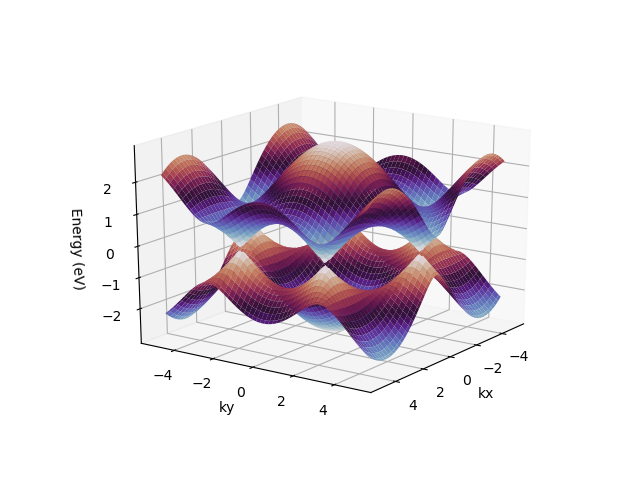
\includegraphics[scale = 0.7]{Graphene_Band_Structure.PNG}
	\caption{Band structure of graphene. Here, $t^{'} = 0$; we can thus see that the bands are symmetric around zero energy. The points where the bands touch are known as \textit{Dirac points}. }
	\label{fig: Graphene Band}
\end{figure}

Consider the tight-binding Hamiltonian for only nearest-neighbor hopping:

\begin{equation}
	H = -t \sum_{<i,j>} \bigg( a_{i}^\dagger b_{j} + h.c. \bigg) 
\end{equation}

Here, the spin index has been removed for clarity. This can be rewritten as:

\begin{equation}
	H = -t \sum_{i\in A} \sum_{\delta} \bigg( a_{i}^\dagger b_{i+\delta} + h.c. \bigg) 
\end{equation}

The sum $\delta$ is carried over the nearest-neighbor vectors $\delta_i$ as shown in Figure \ref{fig: Graphene lattice and FBZ}. We can write the creation operator as:

\begin{equation}
	a_{i}^\dagger = \frac{1}{\sqrt{N/2}} \sum_k e^{i\vec{k}\cdot \vec{r_i}} a_{k}^\dagger
\end{equation}

Here, $N/2$ is the number of A sites; a similar definition applies for $b_{i+\delta}$. Hence, the Hamiltonian can be rewritten as:

\begin{equation}
	H = -t \sum_{\delta, k} \bigg( e^{-i\vec{k}\cdot \vec{\delta}}a_{k}^\dagger b_{k} + h.c. \bigg) 
\end{equation}

Therefore we can write the Hamiltonian in spinor notation:

\begin{align}
	H &= \sum_k \psi^{\dagger}h(\vec{k})\psi \\
	\psi^{\dagger} &= (a_k^{\dagger} \ \ b_k^{\dagger})\\
	h(\vec{k}) &= -t \begin{pmatrix}
				0 & \Delta_k\\
				\Delta_k^{*} & 0
				\end{pmatrix} \\
	\Delta_k &= \sum_{\delta} e^{i\vec{k}\cdot \vec{\delta}}
\end{align}

We can expand $\Delta_k$ as:

\begin{equation}
		\Delta_k = \sum_{\delta} e^{i\vec{k}\cdot \vec{\delta}} = \sum_{\delta} [\cos(\vec{k}\cdot \vec{\delta}) + i\sin(\vec{k}\cdot \vec{\delta})]
\end{equation}

The Hamiltonian can thus also be expressed in terms of Pauli matrices \cite{graphene_tight_bonding}:

\begin{equation}
	h(\vec{k}) = -t \begin{pmatrix}
		0 & \cos(\vec{k}\cdot \vec{\delta}) + i\sin(\vec{k}\cdot \vec{\delta}) \\
		\cos(\vec{k}\cdot \vec{\delta}) - i\sin(\vec{k}\cdot \vec{\delta}) & 0
				\end{pmatrix} 
\end{equation}

\begin{equation}
	h(\vec{k}) = -t \sum_{\delta}[\cos(\vec{k}\cdot \vec{\delta})\sigma_x + i\sin(\vec{k}\cdot \vec{\delta})\sigma_y]
\end{equation}

Written in this form, it is interesting to see what happens if we have a $\sigma_z$ term \cite{graphene_tight_bonding}:

\begin{align}
	h_M (\vec{k}, M) &= -t\sum_{\delta} [\cos(\vec{k}\cdot \vec{\delta})\sigma_x + i\sin(\vec{k}\cdot \vec{\delta})\sigma_y + M\sigma_z]\\
	&= -t \sum_{\delta} \begin{pmatrix}
		M & \cos(\vec{k}\cdot \vec{\delta}) + i\sin(\vec{k}\cdot \vec{\delta}) \\
		\cos(\vec{k}\cdot \vec{\delta}) - i\sin(\vec{k}\cdot \vec{\delta}) & -M
	\end{pmatrix} 
\end{align}

Hence, the additional $\sigma_z$ term raises the energy of A sites and lowers the energy of B sites, thereby gapping the bands; this corresponds to an on-site potential of the form \cite{graphene_tight_bonding}:

\begin{equation}
	H_{potential} = M \bigg( \sum_{\alpha \ \{A \ sites\}} a_{\alpha}^{\dagger}a_{\alpha} - \sum_{\beta \ \{B \ sites\}} b_{\beta}^{\dagger}b_{\beta} \bigg )
\end{equation}

Such a potential arises when there are two different atoms on the A and B sites, such as in boron nitride. In the boron nitride case, the A and B sites correspond to boron and nitrogen atoms.
\newline

The Hamiltonian near the Dirac points with the addition of the $\sigma_z$ term thus takes the form:

\begin{equation}
	h_M = v_F (q_x \sigma_x + q_y \sigma_y + M\sigma_z) = v_F \begin{pmatrix}
					M & q_x -iq_y\\
					q_x + i q_y & -M
					\end{pmatrix}
\end{equation} 

This results in a quadratic dispersion relation:

\begin{equation}
	E_{M, \pm} = \pm \sqrt{q_x^2 + q_y^2 + M^2}
\end{equation} 

This dispersion relation results in the creation of a bandgap, as can be seen in Figure \ref{fig: monolayer_bandgap}.

\begin{figure}[htb]
	\centering
	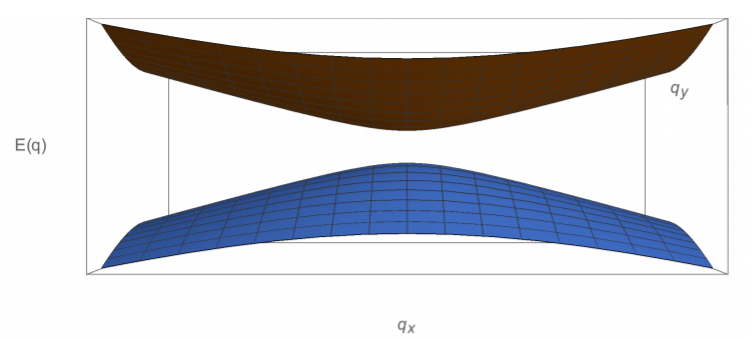
\includegraphics[scale = 0.7]{monolayer_bandgap.PNG}
	\caption{Energy bandgap near a Dirac point produced by a $\sigma_z$ term. Figure and caption have been adapted from \cite{graphene_tight_bonding}.}
	\label{fig: monolayer_bandgap}
\end{figure}


\subsubsection{Density of States}
The full form of the Density of States\footnotemark for the dispersion relation in equation \ref{eq:Full_Band_Equation} can be found in \cite{The_Electronic_Properties_of_Graphene}. Near the Dirac points, this takes the form:
\footnotetext{See Section \ref{sec: DOS} for more information regarding Density of States.}

\begin{equation}
	\rho(E) = \frac{2A_c |E|}{\pi v_F^2}
\end{equation}

Here, $A_c = 3\sqrt{3}a^2/2$ is the unit cell area. As is apparent from Figure \ref{fig: Monolayer_graphene_dos}, monolayer graphene does not permit an energy bandgap, and hence may not necessarily be directly applicable as-is for quantum information applications.

\begin{figure}[htb]
	\centering
	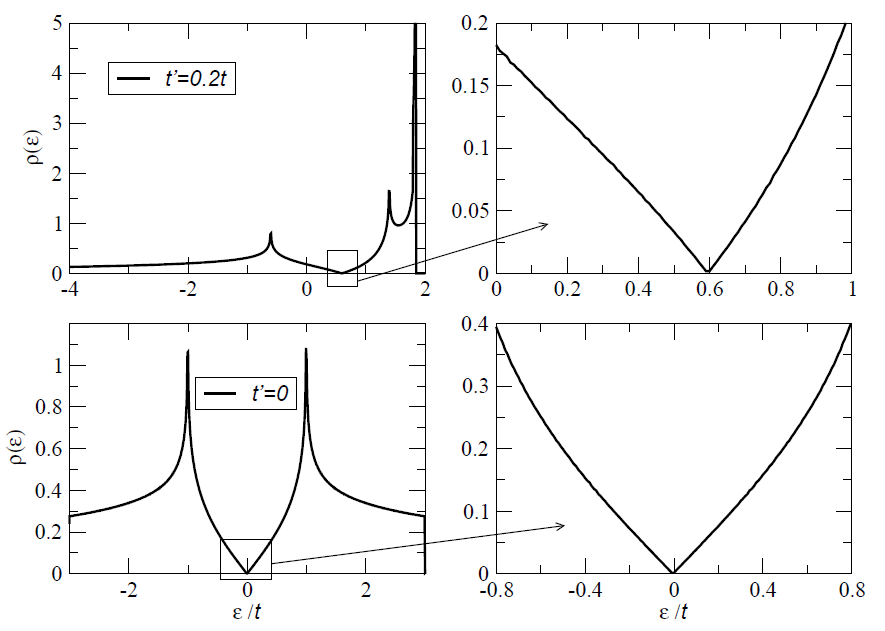
\includegraphics[scale = 0.6]{monolayer_DOS.PNG}
	\caption{Density of states per unit cell as a function of energy (in units of $t$) computed from the energy dispersion relation in \ref{eq:Full_Band_Equation}, $t^{'} = 0.2t$ (top) and for  $t^{'} = 0$ (bottom). Also shown is a zoom in of the density of states close the the neutrality point of one electron per site. For the case  $t^{'} = 0$ the electron-hole nature of the spectrum is apparent and the density of states close to the neutrality point can be approximated by $\rho(\epsilon) \propto |\epsilon|$. Figure and caption are from \cite{The_Electronic_Properties_of_Graphene}. }
	\label{fig: Monolayer_graphene_dos}
\end{figure}


\subsection{Bilayer Graphene}\label{sec: bilayer_graphene}
Bilayer graphene is composed of two monolayer graphene sheets stacked on one another. This presents interesting electrical and optical properties, in particular that of a bandgap between the valence and conduction bands.
\newline

\begin{figure}[htb]
	\centering
	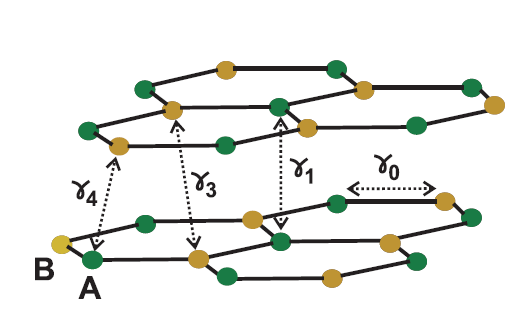
\includegraphics[scale = 0.7]{bilayer_graphene.PNG}
	\caption{ Lattice structure of bilayer graphene, with hopping parameters indicated as $\gamma_i$. Lattice A is indicated by green spheres, and lattice B is indicated by yellow spheres. Figure has been adapted from \cite{The_Electronic_Properties_of_Graphene}. }
	\label{fig: Bilayer_graphene}
\end{figure}

The tight-binding Hamiltonian for bilayer graphene with hopping parameters\footnotemark $\gamma_i$ is \cite{The_Electronic_Properties_of_Graphene}:

\footnotetext{See Figure \ref{fig: Bilayer_graphene} for a visualization of these hopping parameters.}

\begin{align}
	H = -\gamma_0 &\sum_{<i,j>, m, \sigma} \bigg( a_{m, i, \sigma}^\dagger b_{m, j, \sigma} + h.c. \bigg )\\
	-\gamma_1 &\sum_{j, \sigma} \bigg( a_{1, j, \sigma}^\dagger a_{2, j, \sigma} + h.c. \bigg )\\
	-\gamma_3 &\sum_{j, \sigma} \bigg( a_{1, j, \sigma}^\dagger b_{2, j, \sigma} + a_{2, j, \sigma}^\dagger b_{1, j, \sigma} + h.c. \bigg )\\
	-\gamma_4 &\sum_{j, \sigma} \bigg( b_{1, j, \sigma}^\dagger b_{2, j, \sigma, j}  + h.c. \bigg )\\
\end{align}

Here, $a_{m, i, \sigma}$ annihilates an electron with spin $\sigma$ on sublattice A in plane $m = 1, 2$ at site $R_i$, and similarly for $b_{m, i, \sigma}$. The hopping parameters  represent the following \cite{The_Electronic_Properties_of_Graphene}:

\begin{itemize}
	\item $\gamma_0 = t$: In-plane hopping energy.
	\item $\gamma_1$: Hopping energy between atom $A_1$, atom $A_2$; $\gamma_1 \approx 0.4  \ ev$ in graphite.
	\item $\gamma_3 = t$: Hopping energy between atom $A_i$ and atom $B_i$. $\gamma_3 \approx 0.3  \ ev$ in graphite.
	\item $\gamma_4 = t$: Hopping energy connecting atoms $B_1$ and $B_2$. $\gamma_4 \approx -0.04  \ ev$ in graphite.
\end{itemize}

In the continuum limit, the Hamiltonian close to the Dirac points in the Brillouin zone can be written as (ignoring $\gamma_4$):

\begin{align}
	H &= \sum_k \psi_k^{\dagger} \cdot H_K \cdot \psi_k\\
	H_K &= \begin{pmatrix}
			-V &  v_F k & 0 & 3\gamma_3 ak^{*}\\
			v_F k^{*} & -V & \gamma_1 & 0\\
			0 & \gamma_1 & V & v_F k\\
			3\gamma_3 ak & 0 & v_Fk^{*} & V
			\end{pmatrix}
\end{align}

Here, $k \in \mathbb{C}$ is a complex number, and $V$ is half the shift in electro-chemical potential between the two layers (this is in case a potential is applied between the two layers) \cite{The_Electronic_Properties_of_Graphene}. The wavefunction can thus be written as a four-component spinor:

\begin{equation}
	\psi_k^{\dagger} = \bigg ( a_1^{\dagger}(k), \ a_2^{\dagger}(k), \ b_1^{\dagger}(k), \ b_2^{\dagger}(k) \bigg )
\end{equation}

In the case of zero external potential between the two layers ($V=0$) and $\gamma_3, v_F k << \gamma_1$, it is possible to remove high-energy states perturbatively and write an effective Hamiltonian \cite{The_Electronic_Properties_of_Graphene}.

\begin{equation}
	H_{eff} = 
	\begin{pmatrix}
	0 & \frac{v_f^2 k^2}{\gamma_1} + 3\gamma_3ak^{*}\\
	\frac{v_f^2 (k^{*})^2}{\gamma_1} + 3\gamma_3ak & 0	
	\end{pmatrix}
\end{equation}

In the $\gamma_3 = 0$ case, the energy bands derived are parabolic:

\begin{equation}
	E_{k, \pm} \approx \pm v_F^2 k^2 / \gamma_1
\end{equation}

The resulting energy bands are shown in Figure \ref{fig: Bilayer_touching_bands}. Two additional bands are also seen at $\pm \gamma_1$; we can see that this spectrum is electron-hole symmetric. The bilayer can be treated as a metal (zero bandgap), with a constant density of states \cite{The_Electronic_Properties_of_Graphene}. The introduction of the $V$ term breaks inversion symmetry, resulting in the following dispersion relation:

\begin{align}
	E_{\pm, k}^2 &= V^2 + v_F^2 k^2 + \gamma_1^2/2\\
	&\pm \sqrt{4V^2 v_F^2 k^2 + t^2 v_F^2 k^2 + \gamma_1^4/4}
\end{align}

The resulting energy bands are shown in Figure \ref{fig: Bilayer_separate_bands}. Clearly, we see that the addition of the $V$ term introduces a bandgap. The dependence of this bandgap on an external potential $V$, which may be experimentally tuned, makes bilayer graphene useful for technological applications \cite{The_Electronic_Properties_of_Graphene}.


\begin{figure}[htb]
	\begin{subfigure}[b]{0.4\textwidth}
		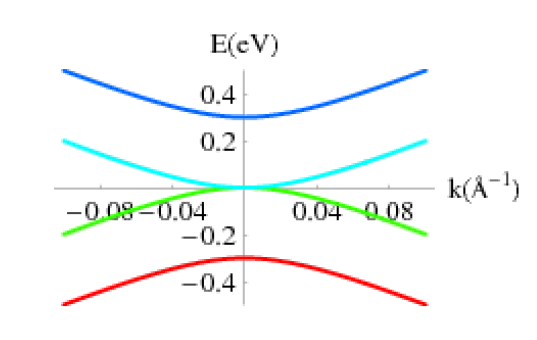
\includegraphics[width=\textwidth]{bilayer_touching_bands.PNG}
		\caption{Band structure for bilayer graphene for $V=0$ and $\gamma_3 = 0$.}
		\label{fig: Bilayer_touching_bands}
	\end{subfigure}
	\hfill
	\begin{subfigure}[b]{0.4\textwidth}
		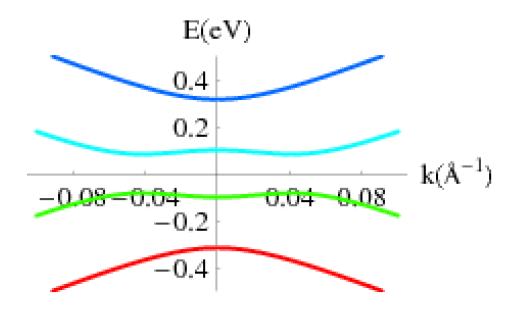
\includegraphics[width=\textwidth]{bilayer_separate_bands.PNG}
		\caption{Band structure for bilayer graphene for $V \neq 0$ and $\gamma_3 = 0$.}
		\label{fig: Bilayer_separate_bands}
	\end{subfigure}
	\caption{Band structure of bilayer graphene in different approximations. Figure and caption have been adapted from \cite{The_Electronic_Properties_of_Graphene}}
\end{figure}

\subsection{Graphene Stacks}
It has been shown experimentally that increasing the number of layers of graphene will result in more metallic behaviour \cite{The_Electronic_Properties_of_Graphene}. Certain types of four-layers stacks of graphene show a bandgap in the presence of charge inhomogeneity between the surface and inner layers, but this does not apply in most cases. Example cases are shown in Figure \ref{fig: graphene_stack_bands}.
\newline

\begin{figure}[htb]
	\centering
	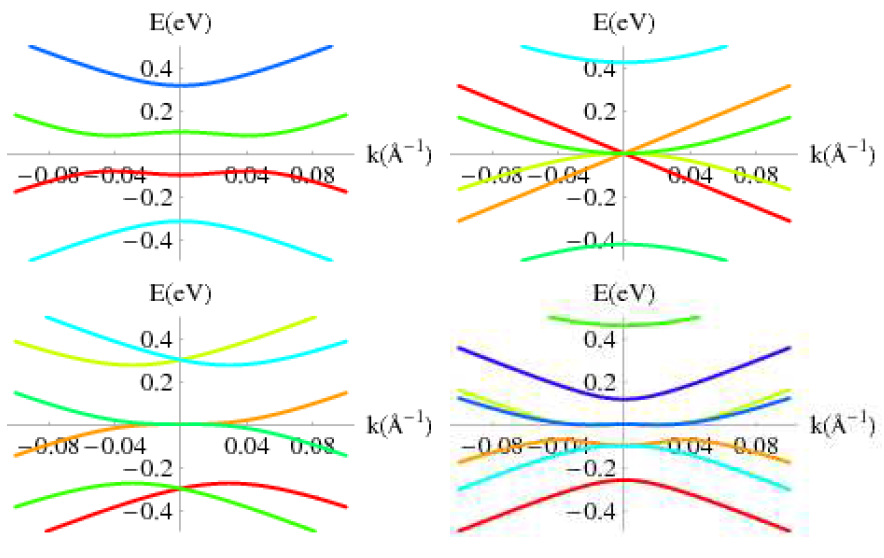
\includegraphics[scale = 0.55]{graphene_stack_bands.PNG}
	\caption{Electronic bands of graphene multilayers: top left: biased bilayer; top right: trilayer with Bernal stacking; bottom left: trilayer with orthorhombic stacking; bottom right: stack with four layers where the top and bottom layers are shifted in energy with respect to the two middle layers by $+0.1 \ eV$. Figure and caption have been adapted from \cite{The_Electronic_Properties_of_Graphene}. }
	\label{fig: graphene_stack_bands}
\end{figure}

It is clear from Figure \ref{fig: graphene_stack_bands} that increasing the amount of layers of graphene stacks results in zero bandgap systems. Hence, they are likely not a viable option for quantum information applications. 


\section{Promising Optical Systems}\label{sec: Promising_Optical_Systems}
Here we look at promising nanoscale optical systems which could serve as reliable single photon emitter sources or spin qubits for quantum information processing applications.
Defect states within such systems must also have a spin, and have good optical properties (see Figure \ref{fig: quantum_emitter_SPS}). Current systems used in research include color centers in diamond and silicon carbide, which feature spin-selective optical transitions, room temperature stability, exceptionally long coherence times, and potential for scalability \cite{Single_defect_emitters_WSe2}. Hence, any system chosen must match or exceed the performance of existing candidates to be viable for quantum information processing applications.

\begin{figure}[htb]
	\centering
	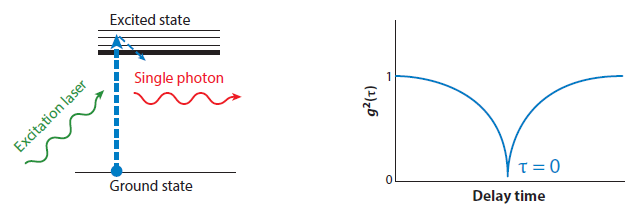
\includegraphics{quantum_emitter_SPS.PNG}
	\caption{Schematic illustration of a single photon emitter operation. \textit{(a)} An isolated quantum system with a ground and an excited state is pumped using a laser (or electrically) and generates a flux of single photons.	\textit{(b)} Schematic illustration of a $g^2(\tau)$ function, with a dip at zero delay time, an indication of a quantum emitter. Figure and caption are from \cite{SP_sources_atomically_thin_materials_review}}
	\label{fig: quantum_emitter_SPS}
\end{figure}

\subsection{Graphene}
Pristine monolayer graphene is not an optimal material for light emission due to its gapless band structure and high conductivity \cite{2D_material_nanophotonics_HBN_BANDGAP, The_Electronic_Properties_of_Graphene}. Point defect states within graphene may be considered as potential single photon quantum emitters (e.g.: graphene fluoride \cite{point_defects_graphene_fluoride}), however research is still being done to explore this possibility. There is potential in this approach, as graphene has a similar crystal structure to hBN, and can accomodate many of the same defects. Additionally, the magnitude of spin-orbit coupling and electron-nuclear spin coupling\footnotemark are both weak in graphene \cite{spinning_edge_graphene, spin_qubits_GQD}, and hence graphene can sustain coherent qubit states. 

\footnotetext{This is partly because natural carbon is made of 99\% \ce{^{12}C} and 1\% \ce{^{13}C} with nuclear spins of 0 and 1/2 respectively, thus resulting in weak coupling to nuclear spin \cite{spin_coherence_GQD_thesis}.}

\subsubsection{Types of Defects in Graphene}

Defects in graphene can be characterized as either intrinsic or extrinsic. The former is composed of non-$sp^2$ orbital hybrid carbon atoms in graphene, whereas the latter are defects that have been introduced into the system (e.g. substitutional impurities) \cite{a_review_on_lattice_defects_in_graphene}. The band dispersion of different defects may vary drastically \cite{band_dispersion_graphene_structural_defects}, hence presenting a variety of potential defect states for applications.
\newline

Intrinsic defects can be further classified as follows \cite{a_review_on_lattice_defects_in_graphene}:

\begin{itemize}
	\item \textbf{Stone-Wales Defects:} Created by the rotation of a single pair of carbon atoms, resulting in adjacent pairs of pentagonal and heptagonal rings \cite{a_review_on_lattice_defects_in_graphene}. The number of carbon atoms in the structure is preserved. The formation energy of this defect is about 5 eV \cite{Stone_Wales_Defect_Formation_Energy}.   
	\item \textbf{Single-Vacancy Defects:} Caused by the removal of a single carbon atom from the lattice. The rest of the lattice is distorted in such a way as to minimize the total energy. The formation energy of this defect is about 7.5 eV \cite{Single_vacancy_defect_formation_energy}. See Chapter 8.3.1 of \cite{Properties_of_graphene:_a_theoretical_perspective} for a detailed DFT analysis of this type of defect.
	
	\item \textbf{Multiple-Vacancy Defects:} Caused by the removal of more than one carbon atom from the lattice, resulting in multiple single-vacancy type defects. The overall lattice may be distorted in such a way as to minimize the total energy, hence resulting in a more stable lattice. 
	
	\item \textbf{Line Defects:} Abnormal grain boundaries may be created due to the process of preparing physics graphene samples (e.g. using chemical vapor deposition, or CVD) \cite{a_review_on_lattice_defects_in_graphene}.
	
	\item \textbf{Carbon Adatoms:} Carbon atoms generated from vacancy-type defects may migrate to other points on the lattice and form new bonds which are outside of the graphene plane. This results in an out-of-plane $sp^3$ bond which effectively makes the structure 3D.
\end{itemize}

Extrinsic defects can also be further classified as follows:

\begin{itemize}
	\item \textbf{Foreign Adatoms:} This subclass of defect can arise either during the preparation of graphene (e.g. CVD; see \cite{synthesis_GNR_metal_oxide} for example), which results in metal atoms or oxygen-containing functional groups to bond to the surface of the graphene sample, or during intentional adsoprtion of adatoms. The latter can also include organic molecules and other functional groups \cite{bandgap_engineering_edge_functionalization_organic, bandgap_tuning_hydrogenated_graphene}.
	
	\item \textbf{Substitutional Impurities:} Carbon atoms in the graphene lattice can be replaced by atoms such as nitrogen and boron, which can form three chemical bonds.
\end{itemize}


\subsubsection{Graphene Nanoribbons}
Graphene nanoribbons (GNRs) are effectively 2D structures, with variable width and macroscopic lengths - i.e. they are narrow strips of graphene. The type of GNR being studied depends on the nature of its edges (i.e. zigzag edge or armchair edge). Consequently, the boundary conditions for both types of edges are different, thereby producing different behaviour at the edges \cite{The_Electronic_Properties_of_Graphene}. See Figure \ref{fig: zizgaz_armchair_GNR} for the types of edges that may be produced in GNRs. These edges give rise to interesting physics, such as localized edge states \cite{bandgap_engineering_GNR_edge_dihydrogenation, Edge_passivation_AGNR_bandgap_engineering, QD_edge_modulated_GNR, Properties_of_graphene:_a_theoretical_perspective}. The energy spectrum for both types of GNR are shown in Figure \ref{fig: armchair_zigzag_energy_bands}.
\newline

\begin{figure}[htb]
	\centering
	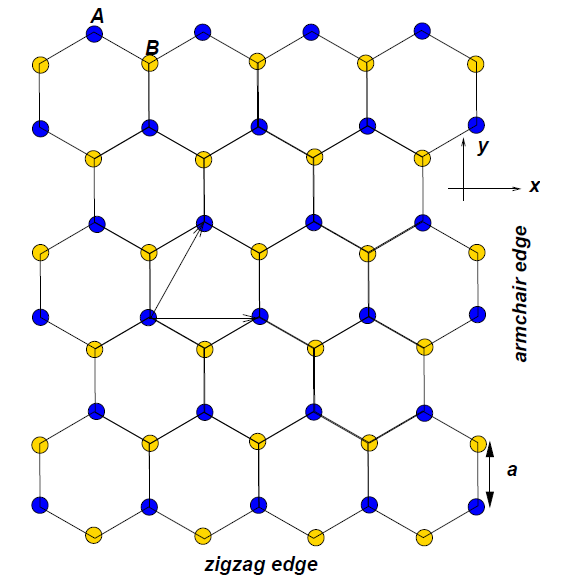
\includegraphics[scale = 0.6]{zigzag_armchair_GNR.PNG}
	\caption{A piece of honeycomb lattice displaying both zigzag and armchair edges. Figure and caption are from \cite{The_Electronic_Properties_of_Graphene}}
	\label{fig: zizgaz_armchair_GNR}
\end{figure}


\begin{figure}[htb]
	\centering
	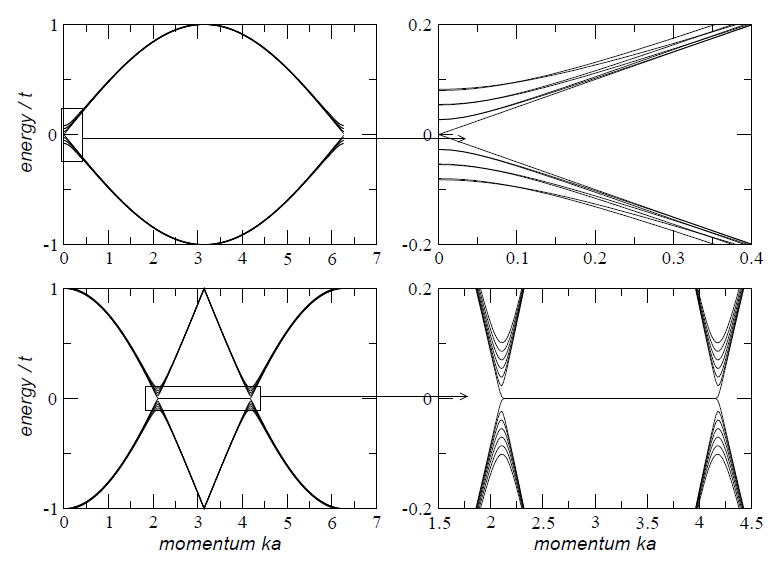
\includegraphics[scale = 0.6]{armchair_zigzag_dispersion.PNG}
	\caption{Left: Energy spectrum, as calculated from the tight-binding equations, for a nanoribbon with armchair (top) and zigzag (bottom) edges. The width of the nanoribbon is N = 200 unit cells. Only fourteen eigenstates are depicted. Right: Zoom of the low energy states shown on the right. Figure and caption are from \cite{The_Electronic_Properties_of_Graphene}}
	\label{fig: armchair_zigzag_energy_bands}
\end{figure}

It may be possible to use nitrogen-vacancy type defects in GNRs as SPEs, however this has mainly been explored in terms of nanoelectronics applications \cite{spin_gapless_N_doped_ZGNR}. Nitrogen and boron were both explored as substitutional dopants in zizgag GNRs, showing the presence of quantum dots \cite{B_N_doped_GNR}. Edge-modulated armchair GNRs were also shown to have optically active quantum dot states, thus being potentially useful for optoelectronic applications \cite{QD_edge_modulated_GNR}. Biexciton states in GNRs also have the potential to be useful in photonics applications \cite{exciton_annihilation_GNR}. Oxygen dopants such as \ce{OH} groups \cite{oxygen_functional_groups_graphene}, as well as radical molecules (on the edges of GNRs) \cite{spinning_edge_graphene} have the potential to be a basis for spin qubits in GNRs, with the latter having spin coherence times on the order of microseconds at room temperature \cite{magnetic_edge_states_coherent_manipulation_GNR}. A downside to the latter implementation is that radical molecules, and in general organic functional groups, tend to be quite large.
\newline

Several studies have been published regarding the bandgap tuning of GNRs. One study showed the magnitude of the bandgap increases continuously to 4.66 eV by partially hydrogenating the graphene lattice \cite{bandgap_tuning_hydrogenated_graphene}. There seems to be an inverse proportionality between the width of GNRs and the size of the bandgap in armchair GNRs \cite{width_depedent_bandgap_AGNR, energy_bandgap_engineering_GNR}. In particular, it was shown in \cite{energy_gaps_armchair_AGNR} that the bandgap decreases as a function of the number of dimer lines across the ribbon width in armchair GNRs. Pristine nanoribbon forms tend to have smaller bandgaps, however manipulation of their atomic edges can lead to larger gaps \cite{bandgap_engineering_GNR_edge_dihydrogenation, Edge_passivation_AGNR_bandgap_engineering}. Graphene nanoribbons will always have dangling bonds in the carbon atoms located at the edges, therefore it is necessary to functionalize them with something; usually, this is hydrogen \cite{bandgap_engineering_GNR_edge_dihydrogenation, Edge_passivation_AGNR_bandgap_engineering}. In \cite{Edge_passivation_AGNR_bandgap_engineering}, it was shown that bandgaps of armchair GNRs varied over a range of 1.6 eV as a function of the \ce{sp^3}-like bonds at the edges. Topological bandgap engineering also provides a means to use topological phases in GNRs to precisely control the bandgap \cite{topological_band_engineering_GNR, engineering_topological_quantum_phases_GNR}. It may be possible to use topological phases in GNRs to induce exotic quantum states such as Majorana fermions, which could serve as qubit sources \cite{engineering_topological_quantum_phases_GNR}. The use of substrates is also a means to control graphene nanoribbon bandgap and the addition of defects \cite{synthesis_GNR_metal_oxide}. Hence, bandgap engineering of GNRs by edge manipulation can lead to desired electronic properties. 
\newline  

Strain engineering also plays a key role in the electronic structure of GNRs. in armchair GNRs, weak uniaxial strain was shown to change the bandgap linearly, but large strain resulted in a periodic oscillation of the bandgap; in zigzag GNRs, strain was found to change the spin polarization at the edges of GNR, thereby modulating the bandgap \cite{bandgap_strained_GNR}. Strain engineering can thus be exploited to achieve desired optoelectronic properties in GNRs.


\subsubsection{Carbon Nanotubes}
Carbon nanotubes (CNTs) can be formed by rolling graphene sheets along one axis \cite{Properties_of_graphene:_a_theoretical_perspective}. CNTs display strong excitonic binding, extremely narrow linewidth ($\sim$0.1 meV), long coherence times, and have a broad emission spectrum (between 850nm and 2 $\mu$m), however have low quantum yield, low indistinguishability, and high sensitivity to spectral diffusion and blinking \cite{CNT_emerging_quantum_light_source}. Functionalization of CNTs using complex molecular dopants allows the ability to tune the optoelectronic properties of CNTs \cite{CNT_emerging_quantum_light_source, tunable_room_temp_SPE_CNTs}. Room temperature SPEs based on aryl dopants in CNTs operating at telecom wavelengths were shown to have ultrahigh purity (99\%) and high emission rates ($10^5$-$10^7 \ s^{-1}$) \cite{tunable_room_temp_SPE_CNTs}. Doped CNTs in a \ce{SiO_2} substrate were shown to have SPEs operating in telecom wavelengths with nanosecond dopant state lifetimes and good photoluminescence properties at room temperature \cite{room_temp_dopants_CNT}. Additionally, oxygen dopants in CNTs seem to be a promising SPE source \cite{oxygen_dopants_cnts}.


\subsubsection{Graphene Quantum Dots}
Quantum dots (QDs) generally consist of bound excitons confined to zero dimensions by an external potential, generated by either local strain and/or a crystallographic defect \cite{SP_sources_atomically_thin_materials_review}. In general, we expect very long coherence times for graphene spin qubits as both the spin–orbit coupling and the hyperfine interaction are known to be weak in carbon \cite{spin_qubits_GQD, spin_coherence_GQD_thesis, QD_spin_qubits_graphene}.
\newline

Spin qubits with long coherence times have been shown to exist in graphene QDs with armchair boundaries \cite{spin_qubits_GQD}. Graphene QDs have also been shown to have stable single-photon emitters, good brightness and photostability at room temperature \cite{SPE_QD_room_temp}. Various topologies can serve as graphene QDs, such as GNRs and discs \cite{QD_spin_qubits_graphene}. 
\newline

However, there seems to be no evidence of narrow photoluminescence lines at room temperature. Additionally, graphene QDs are not atomic-scale defects, hence may not be entirely relevant for our purpose.

\subsection{Hexagonal Boron Nitride}

Hexagonal boron nitride (hBN) is a wide-bandgap semiconductor ($\sim$6 eV \cite{2D_materials_for_quantum_information_science, hBN_cavity_optomechanics, SP_sources_atomically_thin_materials_review}) with a broad range of single photon emitters (SPEs) with zero phonon line (ZPL) energies in the NIR-visible range ($\sim$1.6–2.2 eV) and the UV range ($\sim$4.1 eV) \cite{SP_sources_atomically_thin_materials_review, ultrviolet_SPE_hBN}. However, ZPL energies in hBN defect emitters tend to be random between the range of $\sim$ 1.5 to 2.2 eV, with the ZPL width scaling exponentially with temperature \cite{SP_sources_atomically_thin_materials_review}. hBN has several defect states that enable room-temperature SPEs \cite{carbon_source_SPE_hBN, first_principles_quantum_emission_hBN, hBN_cavity_optomechanics, quantum_emission_hBN_monolayers, spin_defects_hBN, structural_electronic_properties_hBN}. For instance, the negatively charged boron vacancy center ($VB^{-}$) is a promising spin qubit candidate \cite{spin_defects_hBN, ab_initio_VBneg_hBN}, and the $C_B V_N$ defect (carbon atom substitutes a boron atom and the opposite nitrogen atom is removed) displays good experimental photoluminescence lineshape \cite{first_principles_quantum_emission_hBN}. The $V_B C_N$ defect was also predicted to have a triplet ground state, making it interesting for quantum-qubit operations \cite{hBN_Triplet_GS}. Other defects include nitrogen and boron vacancies \cite{quantum_emission_hBN_monolayers, spin_defects_hBN, ab_initio_VBneg_hBN} and nitrogen \cite{hBN_Triplet_GS}, carbon \cite{carbon_source_SPE_hBN, defective_graphene_domains_hBN}, and oxygen impurities \cite{SPE_Plasma_treated_hBN, SP_sources_atomically_thin_materials_review}.
\newline

SPEs in hBN in the NIR and visible spectrum exhibit exceptional brightness ($> 10^6  \ Hz$ in the absence of Purcell enhancements) linear in-plane polarization, weak electron-phonon coupling (small phonon sidebands) and exceptional photostability \cite{SP_sources_atomically_thin_materials_review}. They also display a higher Debye-Waller factor (ratio of ZPL intensity to total emission) at around $\sim$0.82 compared to $\sim$0.13 for NV centers \cite{2D_materials_for_quantum_information_science}. Experimentation has showed that emitters have the tendency to form near the grain boundaries and flake edges, however this is not a universal characteristic \cite{SP_sources_atomically_thin_materials_review}. However, emitters in hBN have shown to be susceptible to spectral diffusion, thereby affecting indistinguishability of photons \cite{SP_sources_atomically_thin_materials_review}.
\newline


Strain engineering has also been used to tune the properties of hBN defects. For instance, tensile and compressive strain can induce wavelength shifts of SPEs \cite{SP_sources_atomically_thin_materials_review}. Strain-sensitivity can also partially account for wide spectral diffusion in SPEs. Furthermore, strain engineering has also been used experimentally \cite{tunable_bandgap_2d_hBN} and theoretically \cite{first_principles_strain_induced_energy_gaps_BN_graphene_bilayers} to tune the bandgap of hBN defects.


\begin{figure}[h!tb]
	\centering
	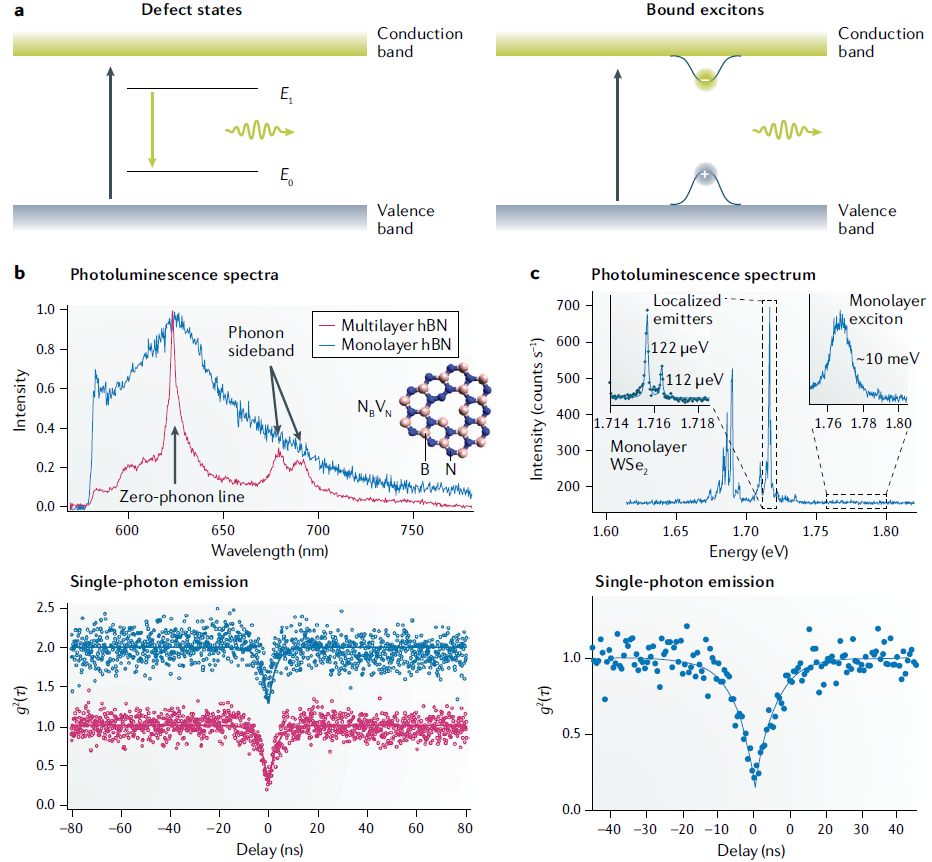
\includegraphics[width = \textwidth]{hbn_properties.PNG}
	\caption{\textbf{Single-photon emitters in 2D materials.} \textbf{a} | Schematic representation of photoluminescence from deep in-gap states (colour centres) in a wide-gap insulator (such as hexagonal boron nitride, hBN) and from bound excitons in a narrow-gap semiconductor (such as \ce{MoS_2}). $E_0$ and $E_1$ are the ground state and first excited state, respectively , of the colour centre. \textbf{b} | Photoluminescence spectra and single-photon emission from monolayer and multilayer hBN (top).	The inset shows the \ce{N_B V_N} defect structure, in which a nitrogen atom substitutes for boron, with a vacancy on the nitrogen site. The emission lines from multilayer samples are narrower than those from monolayer samples. For both	types of samples, the defects act as single-photon emitters, as demonstrated by the antibunching curves (bottom). \textbf{c} | Photoluminescence (top) and single-photon emission (bottom) from monolayer \ce{WSe_2}. The insets in the top panel are zoomed-in spectra of zero-phonon lines and delocalized exciton photoluminescence; the spectrum on the right is integrated for 60 s, the spectrum on the left for 1 s. Figure and caption are from \cite{2D_materials_for_quantum_information_science}.}
	\label{fig: hbn_properties}
\end{figure}

\subsection{Transition Metal Dichalcogenides}
Transition metal dichalcogenides (TMDCs) are 2D semiconductor materials with unique electrical, mechanical, and optical properties \cite{synthesis_TMDC}. TMDCs have the general chemical formula \ce{MX_2}, where \ce{M} is a transition metal and \ce{X} is a chalcogen element (S, Se, Te) \cite{electronic_properties_2D_materials_TMDCs}. TMD monolayers (e.g. \ce{MoS_2}, 
\ce{WS_2}, \ce{MoSe_2}, \ce{WSe_2}) possess a direct bandgap of $\sim$1-2 eV; TMDC bilayers and multilayers possess an indirect bandgap \cite{electronic_properties_2D_materials_TMDCs, 2D_material_nanophotonics_HBN_BANDGAP}. The bandgaps of TMDC monolayers are generally smaller than that of hBN and direct, thus providing efficient generation of excitons upon optical excitation \cite{2D_materials_for_quantum_information_science}. Strong spin-orbit coupling from transition metals may be useful for optoelectronic applications \cite{2D_material_nanophotonics_HBN_BANDGAP}. 
\newline


TMDC monolayers are also good candidates for strain-tunable bandgaps, which can be tuned to engineer the optoelectronic response of the materials for specific applications \cite{electronic_properties_2D_materials_TMDCs, 2D_material_nanophotonics_HBN_BANDGAP, 2D_materials_for_quantum_information_science}.
\newline

SPEs in TMDCs have the ability to be electrically triggered (i.e. electroluminescence) \cite{2D_materials_for_quantum_information_science}. Excitons in \ce{WSe_2} which act as SPEs display good optical properties, however this is only at cryogenic temperatures \cite{2D_materials_for_quantum_information_science}. SPEs have also been shown to exist in \ce{WS_2}, \ce{WSe_2}, \ce{GaSe}, \ce{MoS_2} and \ce{MoSe_2} \cite{2D_materials_for_quantum_information_science, Single_quantum_emitters_monolayer_semiconductors_WSe2_MoS2, Single_defect_emitters_WSe2, WSe2_QE_hBN, SPE_silicon_nitride_photonic_chip, WS2_electrically_driven_photon_emission, SPE_GaSe}. In general, SPEs in TMDCs are currently limited to cryogenic temperatures, therefore limiting their applications to room-temperature quantum network applications; additionally, a broad fluorescence background that overlaps with the quantum
emitter lines necessitates the use of efficient narrow band filters to achieve high photon purity \cite{SP_sources_atomically_thin_materials_review}. Figures \ref{fig: TMDC_table} and \ref{fig: TMDC_hBN_band_emission_properties} show properties of two-dimensional nanophotonic platforms and their optical and band properties.

\begin{figure}[htb]
	\centering
	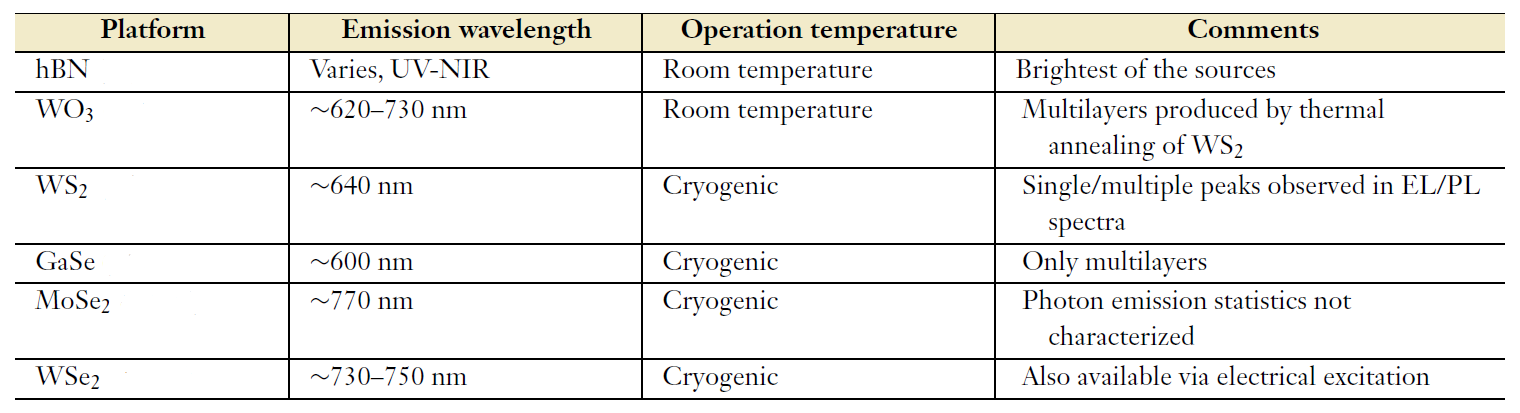
\includegraphics[width = \linewidth]{TMDC_table.PNG}
	\caption{Various two-dimensional material systems that host single photon emitters. Figure and caption are from \cite{SP_sources_atomically_thin_materials_review}}
	\label{fig: TMDC_table}
\end{figure}

\begin{figure}[htb]
	\centering
	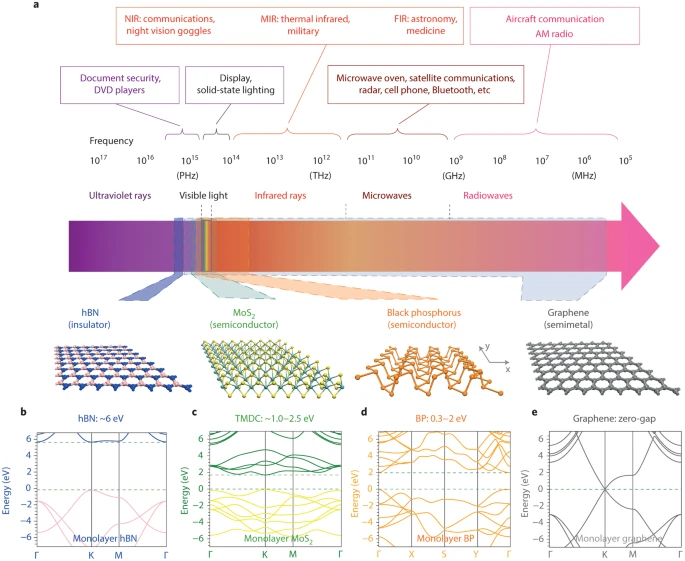
\includegraphics[width = \linewidth]{TMDC_hBN_band_emission_properties.PNG}
	\caption{Various two-dimensional material systems that host single photon emitters. Figure and caption are from \cite{2D_material_nanophotonics_HBN_BANDGAP}}
	\label{fig: TMDC_hBN_band_emission_properties}
\end{figure}

\subsubsection{Tungsten Diselenide}
\ce{WSe_2} has a direct bandgap of $\sim$1.7 eV \cite{SP_sources_atomically_thin_materials_review}. The SPEs in \ce{WSe_2} are predominantly NIR QDs attributed to bound excitons localized by strain fields \cite{SP_sources_atomically_thin_materials_review, WSe2_QE_hBN, SPE_silicon_nitride_photonic_chip}. Excited state lifetimes and emission line widths are on the order
of 2 ns and 100 $\mu$eV, respectively \cite{SP_sources_atomically_thin_materials_review, Single_quantum_emitters_monolayer_semiconductors_WSe2_MoS2}. Emitters in \ce{WSe_2} typically decorate flake edges and extended defects such as scratches, wrinkles/
folds, and nanobubbles; this is typically attributed to strain fields \cite{SP_sources_atomically_thin_materials_review}. Deposition of \ce{WSe_2} layers onto substrates also affect the excited state lifetime, emission line width, and spectral diffusion characteristics \cite{SP_sources_atomically_thin_materials_review, SPE_silicon_nitride_photonic_chip, WSe2_QE_hBN}. Figure \ref{fig: hbn_properties} shows the photoluminescence spectrum and single photon emission properties ($g^2$ function) for exciton-based SPEs.

\subsubsection{Molybdenum Disulfide}
\ce{MoS_2} has been shown to have large spin-orbit coupling, leading to hybrid valley qubits with large coherence times with the potential for optical readout \cite{2D_materials_for_quantum_information_science, SP_sources_atomically_thin_materials_review}. Most of these implementations are quantum dots, however, so they are not atomic-scale defects. In particular, it was shown in \cite{MOS2_properties} that 2D nanostructures in \ce{MoS_2} exhibit good magnetic properties at room temperature, hence being potentially useful for quantum information applications. \ce{MoS_2} has been shown to have an optical bandgap exceeding 1 eV \cite{2D_material_nanophotonics_HBN_BANDGAP}.

\subsubsection{Additional TMDC Systems}

Additional TMDCs which exist but were not explored extensively in this report include \ce{GaSe} \cite{SPE_GaSe}, \ce{WS_2} \cite{WS2_electrically_driven_photon_emission}, \ce{WTe_2} \cite{WTe2_point_defects_influence}, \ce{MoSe_2} \cite{SP_sources_atomically_thin_materials_review, 2D_material_nanophotonics_HBN_BANDGAP}, and \ce{WO_3} \cite{SP_sources_atomically_thin_materials_review}.


\section{DFT Simulations}\label{sec: DFT_simulations}
\subsection{Optical Defect Requirements}\label{sec: Optical_Defect_Requirements}
Ideally, our goal is to find an optically active defect in graphene which may be useful for quantum network applications. In particular, we require photons emitted from defect states to have a minimum energy of 0.8 eV, which corresponds to a wavelength of around 1.5 $\mu m$. Additionally, the defect states must not be too close to the band edges, or else there may be problems due to phonon excitations, especially at room temperature. There must also be two states of the defect, a ground and excited state, with the ground state also having a spin. These requirements guide our search of optical defects in graphene. 

\subsection{Method}
The freely available DFT software \textit{Quantum Espresso} (QE) was used to perform calculations \cite{quantum_espresso}. A graphical user interface for QE, called \textit{BURAI} \cite{Burai}, was also used to simplify the process of defining the supercell and specifying calculation parameters. Calculations made in \textit{BURAI} were limited to energy band and DOS calculations based on user-specified geometries, however, due to the complexities of performing calculations to predict spin properties\footnotemark (e.g. hyperfine coupling, zero-field splitting). All DFT pseudopotentials used were downloaded from the QE website. CIF files specifying the positions of atoms are available at \cite{QE_Google_Drive}.

\footnotetext{See \cite{first_principle_dft_spin_qubits_diamond} for an example of how spin-defect related properties in diamond were calculated using first principles DFT calculations.}

\subsection{Hexagonal Boron Nitride}
We first need to confirm the accuracy of calculations made in Quantum Espresso. To do this, we first compute the DOS and band structure of hexagonal boron nitride (hBN):


\begin{figure}[H]
	\centering
	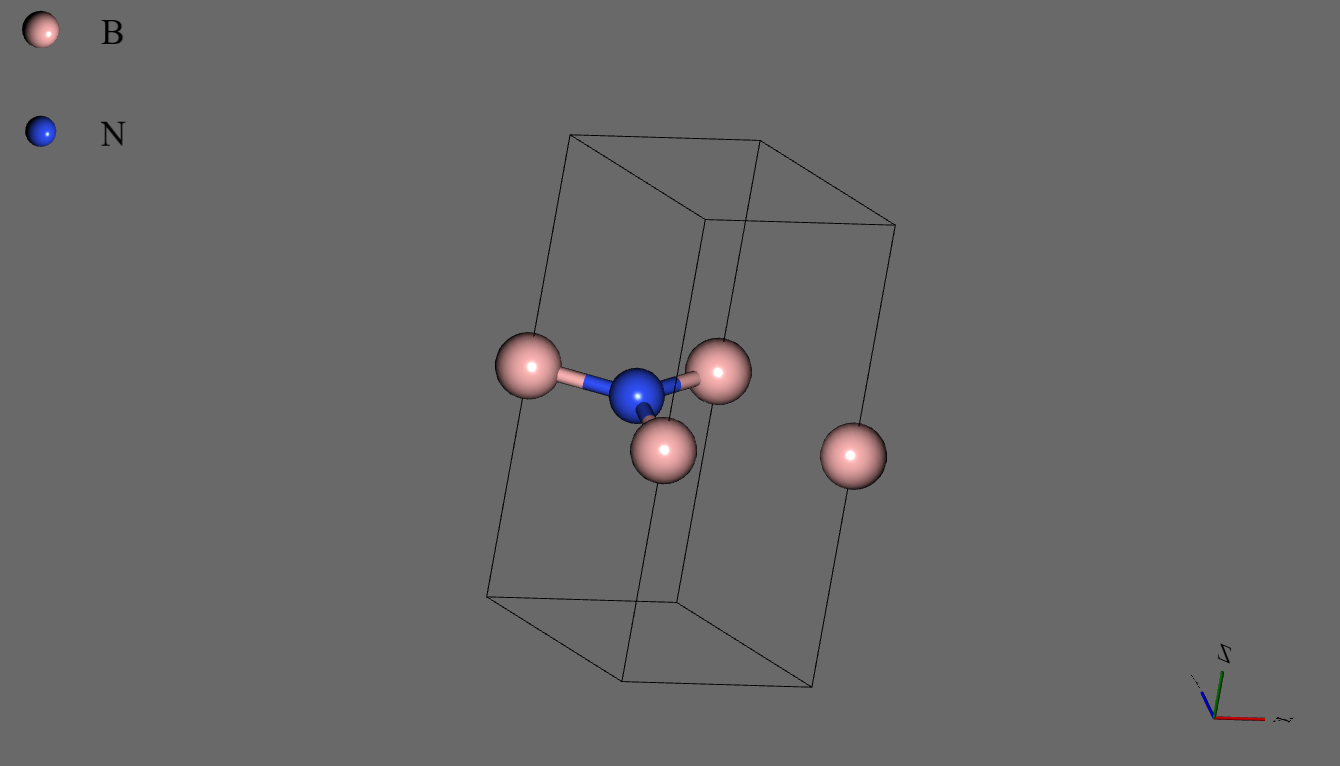
\includegraphics[width = \textwidth]{hbn_geometry.PNG}
	\caption{hBN geometry in \textit{BURAI}.}
	\label{fig: hBN_geometry}
\end{figure}

The unit cell geometry used is shown in Figure \ref{fig: hBN_geometry}. This structure is repeated periodically in the plane to form a two-dimensional crystal structure.

\begin{figure}[H]
	\centering
	\begin{subfigure}[b]{\textwidth}
		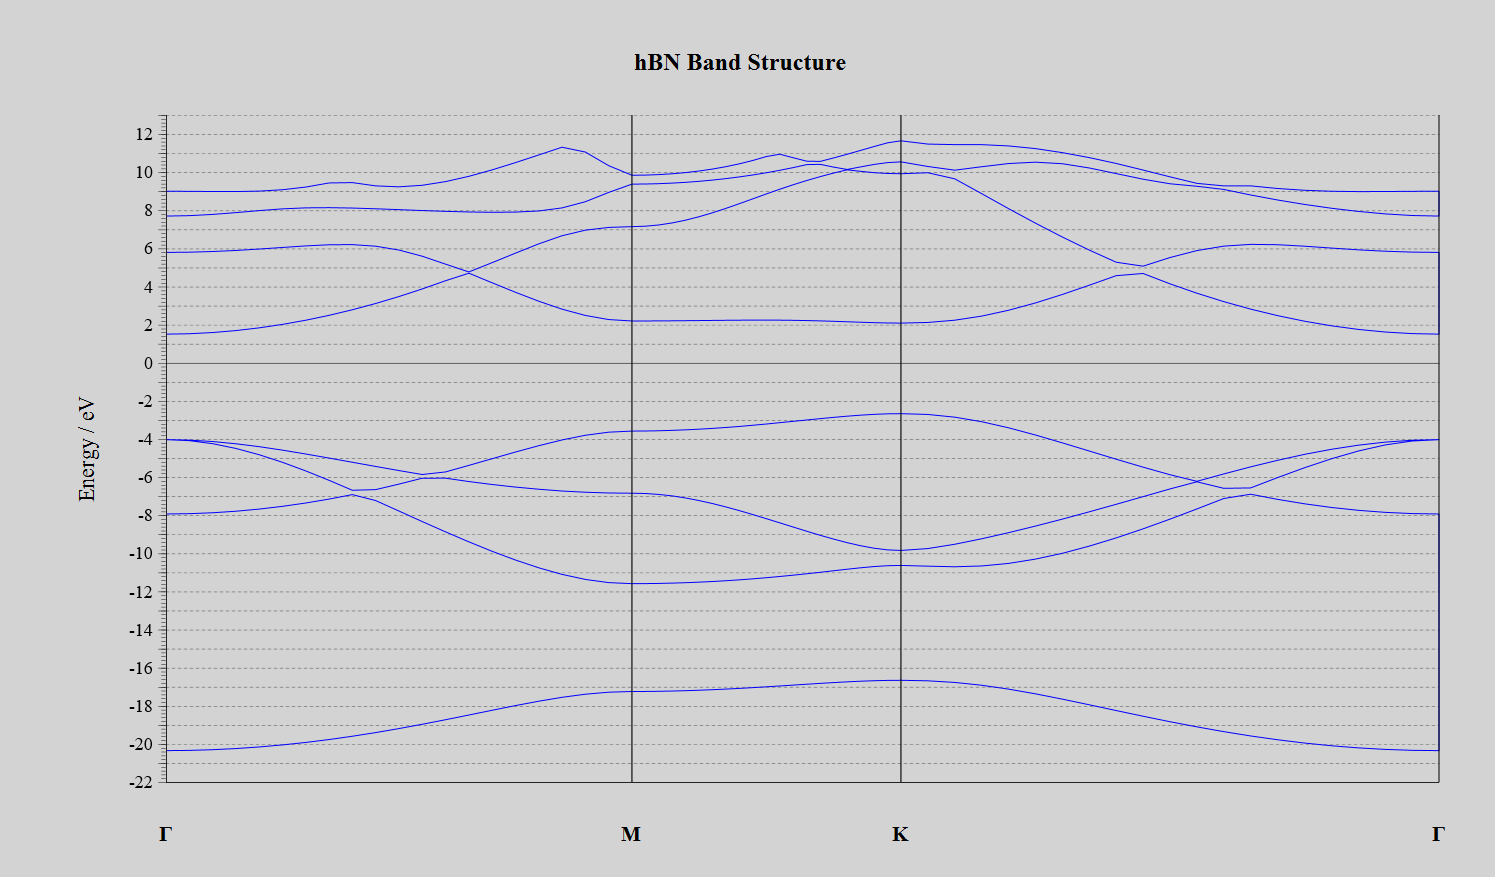
\includegraphics[width = \textwidth]{hbn_band.PNG}
		\label{fig: hbn_band}
	\end{subfigure}
	\hfill
	\begin{subfigure}[b]{\textwidth}
		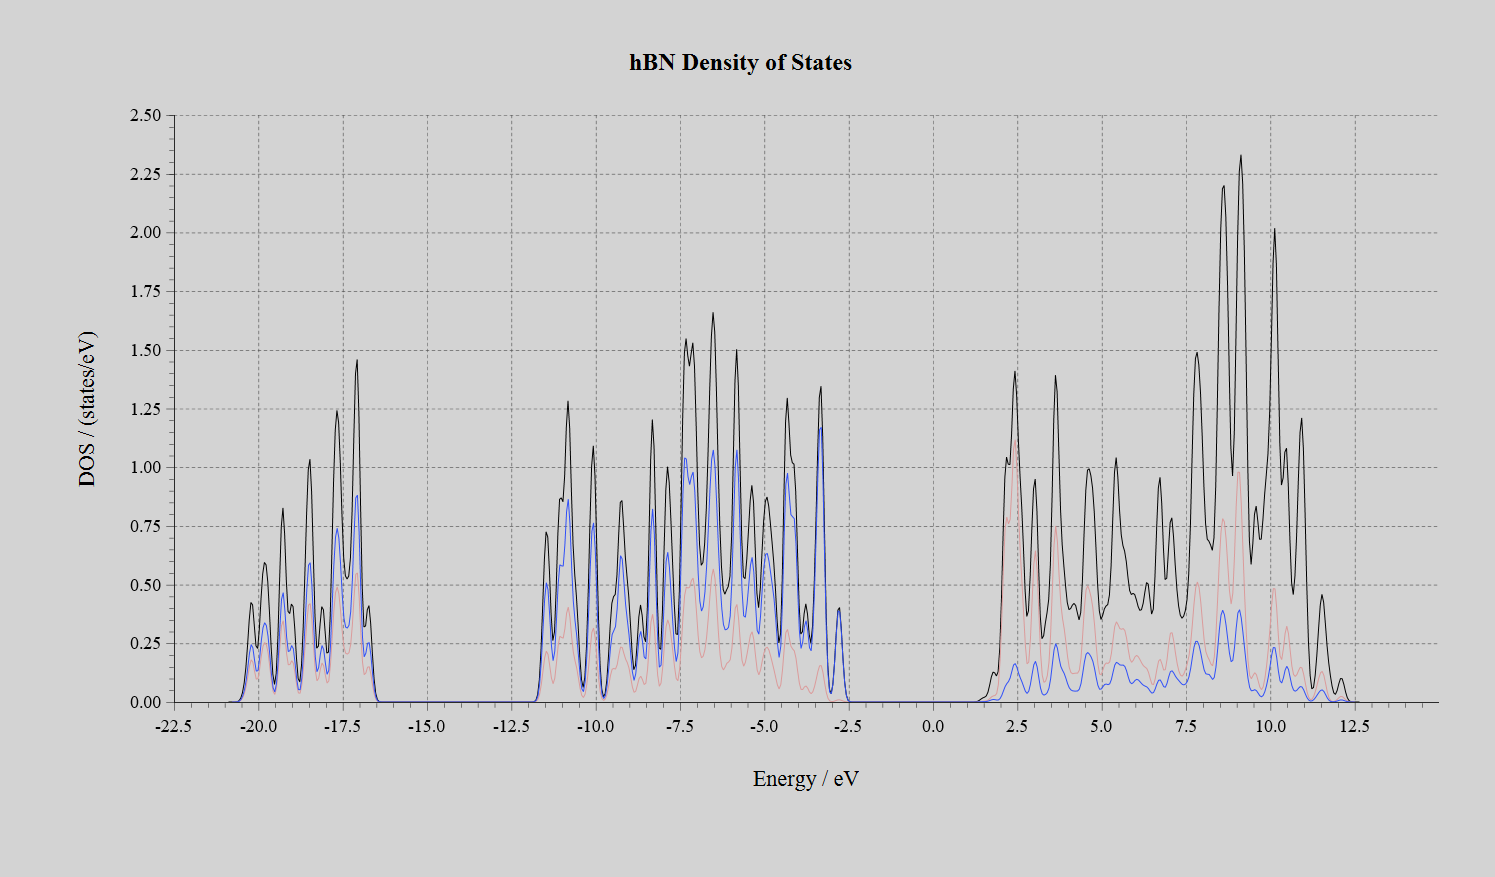
\includegraphics[width = \textwidth]{hbn_dos.PNG}
		\label{fig: hbn_dos}
	\end{subfigure}
	\caption{Band structure (top) and DOS (bottom) of hBN. Pink and blue lines in the DOS diagram represent contributions from boron and nitrogen, respectively. }
	\label{fig: hbn_dos_band}
\end{figure}


We can see from Figure \ref{fig: hbn_dos_band} that the bandgap is about 4.5 eV, which is consistent with the literature on monolayer 2D hBN \cite{tunable_bandgap_2d_hBN, quantum_emission_hBN_monolayers, 2D_material_nanophotonics_HBN_BANDGAP, hBN_cavity_optomechanics}. 


\newpage
\subsection{Graphene}
\subsubsection{Monolayer Graphene}

The monolayer graphene band structure can be seen in Figure \ref{fig: monolayer_graphene_band_dos}.

\begin{figure}[H]
	\centering
	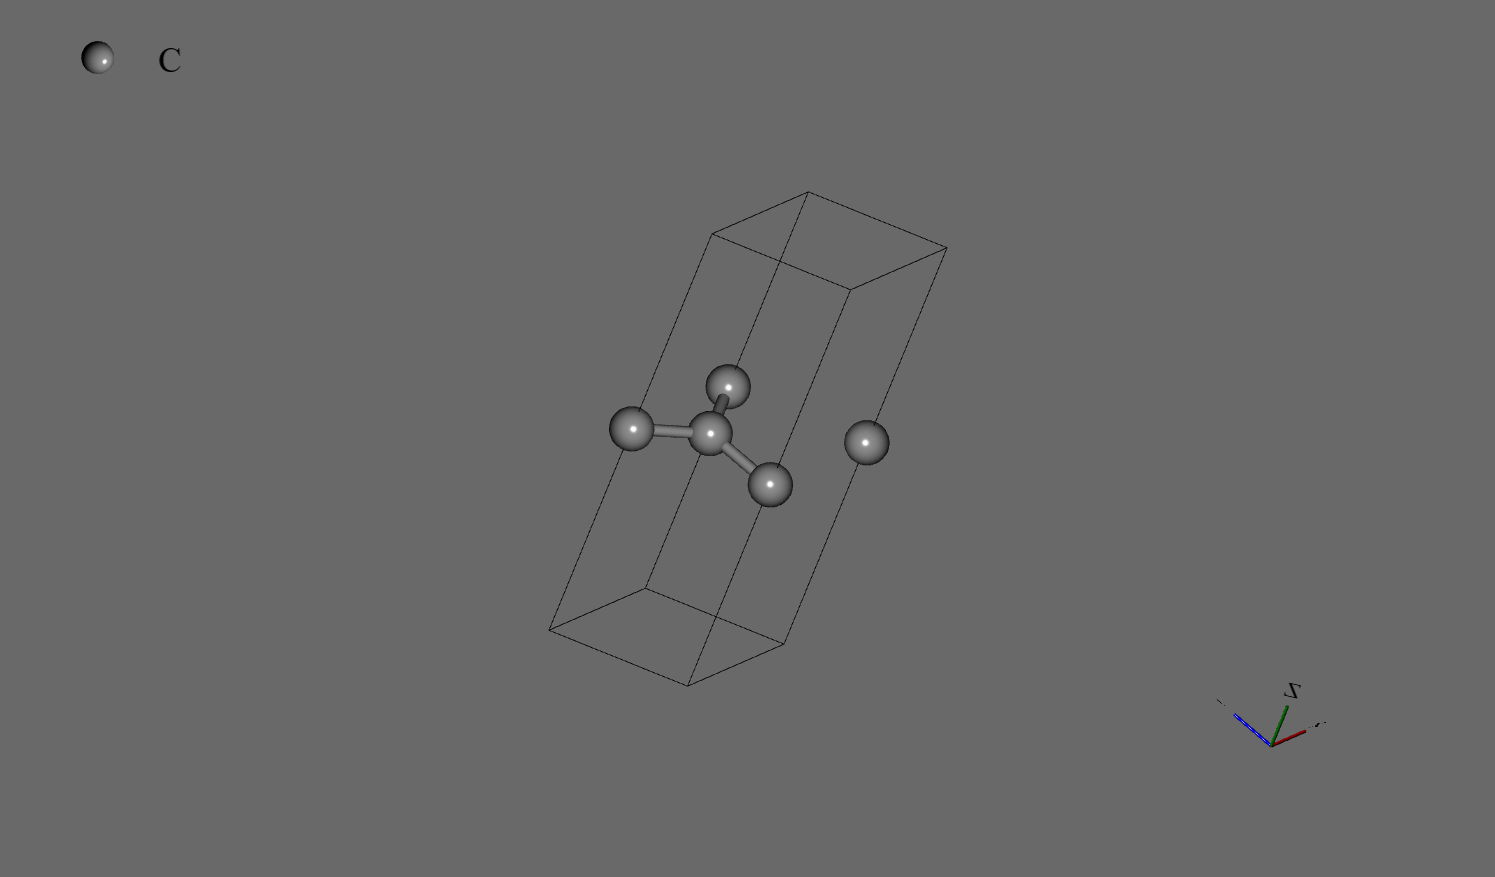
\includegraphics[width = \textwidth]{monolayer_graphene_geometry.PNG}
	\caption{Monolayer graphene geometry in \textit{BURAI}.}
	\label{fig: monolayer_graphene_geometry}
\end{figure}


\begin{figure}[H]
	\centering
	\begin{subfigure}[b]{\textwidth}
		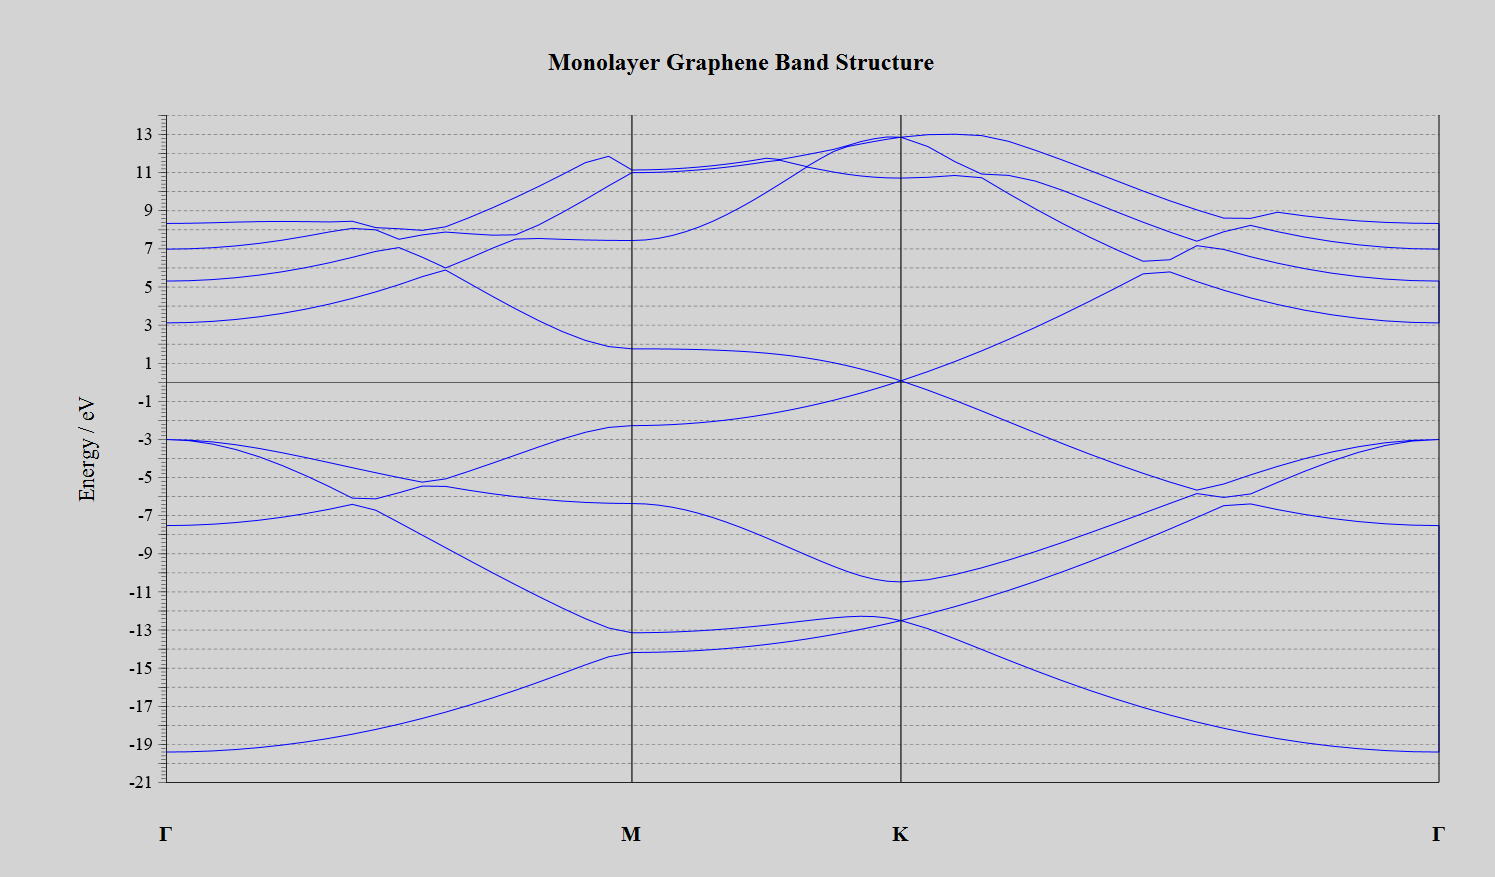
\includegraphics[width = \textwidth]{monolayer_graphene_band.PNG}
		\label{fig: monolayer_graphene_band}
	\end{subfigure}
	\hfill
	\begin{subfigure}[b]{\textwidth}
		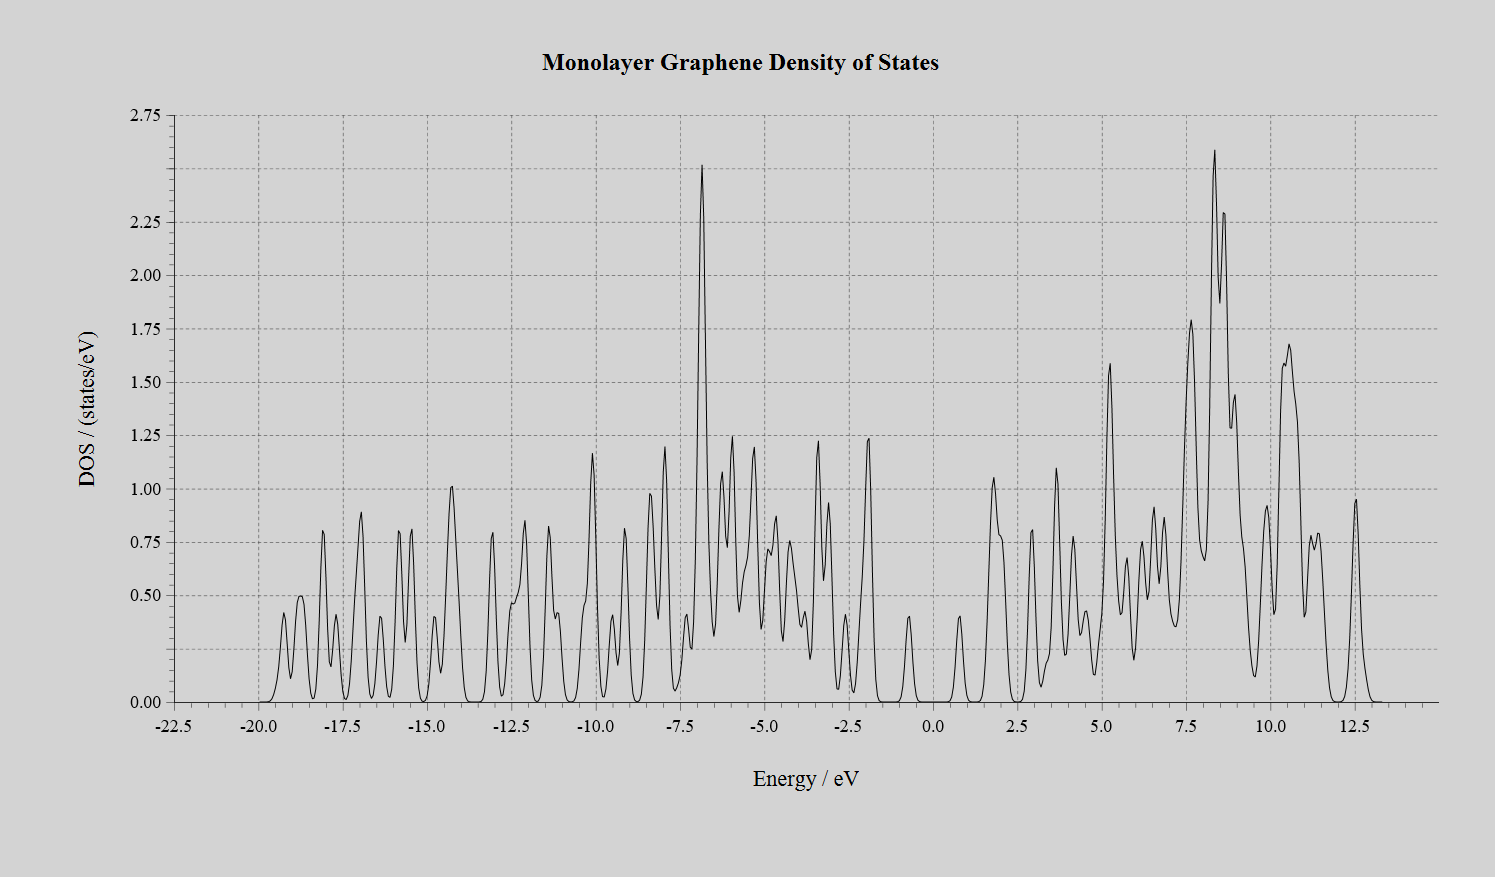
\includegraphics[width = \textwidth]{monolayer_graphene_dos.PNG}
		\label{fig: monolayer_graphene_dos}
	\end{subfigure}
	\caption{Band structure (top) and DOS (bottom) of monolayer graphene. }
	\label{fig: monolayer_graphene_band_dos}
\end{figure}

We can see the presence of the Dirac cones at the K point from the band structure in Figure \ref{fig: monolayer_graphene_band_dos}. This result is in agreement with the literature for monolayer graphene \cite{The_Electronic_Properties_of_Graphene, Properties_of_graphene:_a_theoretical_perspective}.


\newpage
\subsubsection{Bilayer Graphene}

The bilayer graphene band structure can be seen in Figure \ref{fig: bilayer_graphene_band_dos}.

\begin{figure}[H]
	\centering
	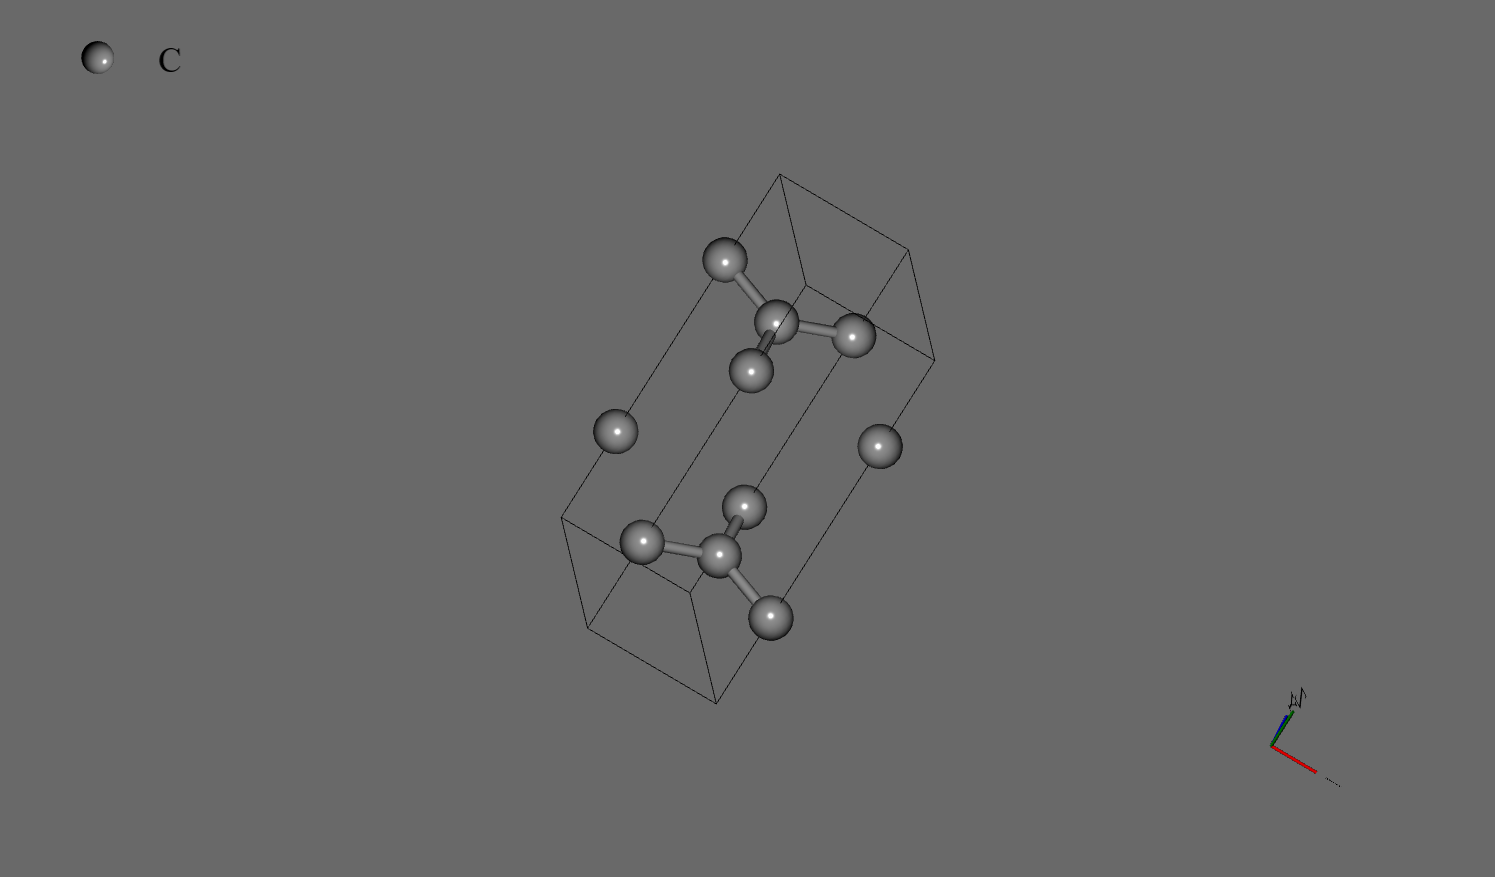
\includegraphics[width = \textwidth]{bilayer_graphene_geometry.PNG}
	\caption{Bilayer graphene geometry in \textit{BURAI}.}
	\label{fig: bilayer_graphene_geometry}
\end{figure}


\begin{figure}[H]
	\centering
	\begin{subfigure}[b]{\textwidth}
		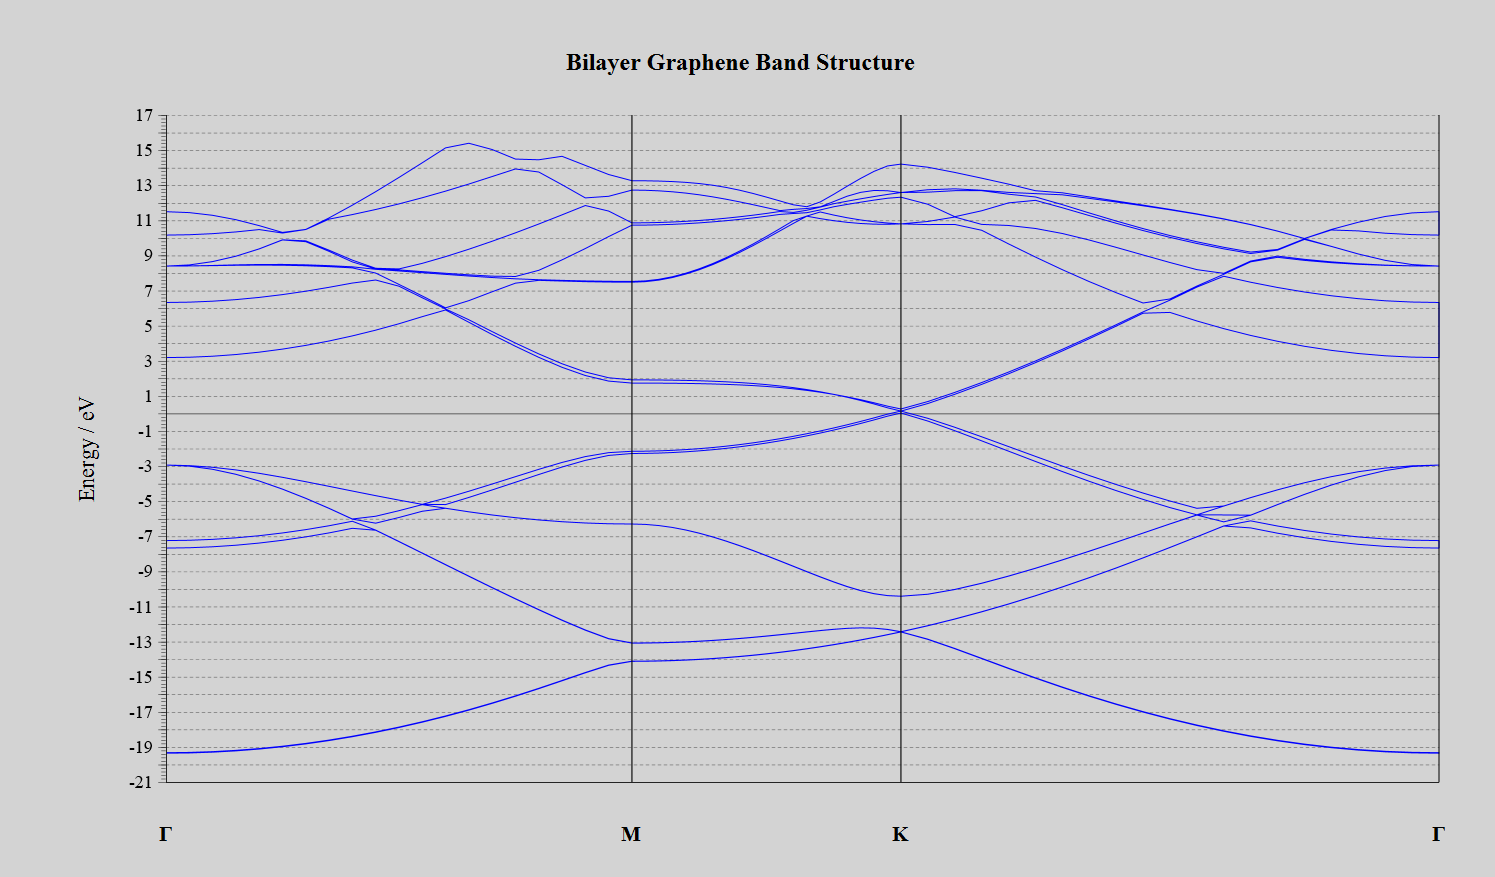
\includegraphics[width = \textwidth]{bilayer_graphene_band.PNG}
		\label{fig: bilayer_graphene_band}
	\end{subfigure}
	\hfill
	\begin{subfigure}[b]{\textwidth}
		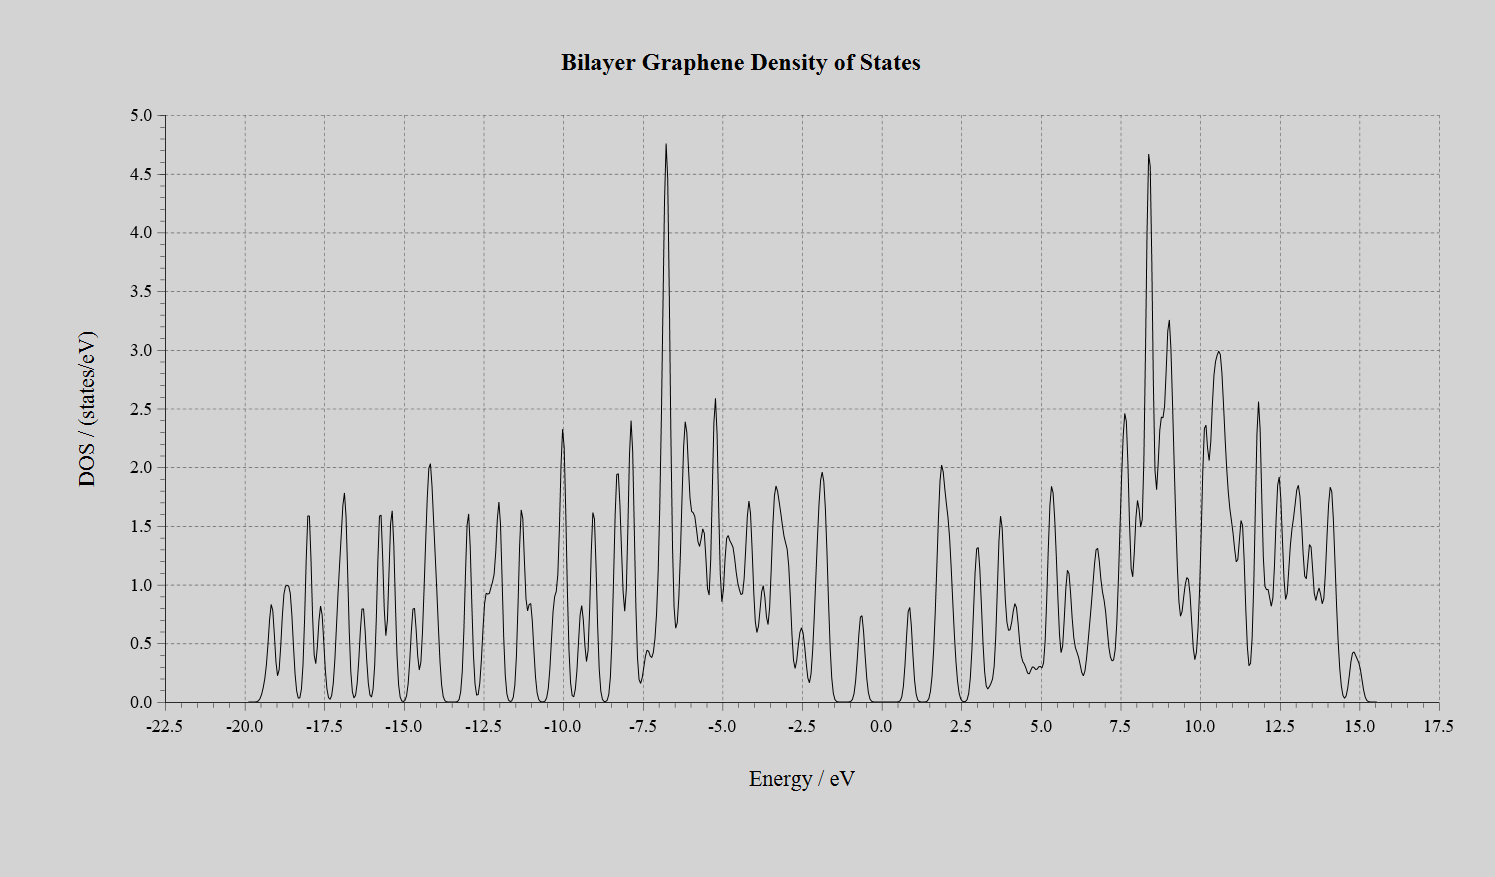
\includegraphics[width = \textwidth]{bilayer_graphene_dos.PNG}
		\label{fig: bilayer_graphene_dos}
	\end{subfigure}
	\caption{Band structure (top) and DOS (bottom) of bilayer graphene. }
	\label{fig: bilayer_graphene_band_dos}
\end{figure}

The DOS and band structure diagrams of bilayer graphene seem to be very similar qualitatively to the monolayer graphene DOS and band structure diagram in Figure \ref{fig: monolayer_graphene_band_dos}. The gapless bilayer structure may be tuned by an external potential or strain to induce a bandgap, as was discussed in Section \ref{sec: bilayer_graphene}.



\newpage
\subsection{Issues Regarding Band Folding}
See the following excerpt from \cite{band_folding_thesis} regarding the issue of band folding when performing DFT calculations:
\newline

''\textit{In typical band structure calculations, only a primitive cell of the structure is considered, which is then used to populate the bulk structure and leads to the well known
E-k diagrams. However, it is very difficult to truly represent anything other than a
perfect structure within a primitive cell due to the perfect symmetry forced upon the
system. Therefore, structures larger than a primitive cell need to be explored in order
to accurately reproduce the effect of defects like the random nature in the distribution
of atomic species and position. A method to calculate the band structure of this larger
structure is called the supercell approach. This maintains the symmetrical effects of the
primitive cell, so can be repeated infinitely to produce a bulk structure but does so from
a much larger base.}
\newline

\textit{A supercell is generally built from multiple non-identical primitive cells stacked along
their lattice vectors that results in a shape that is capable of being tessellated. The
supercell structure will then need to be relaxed so that the structure is continuous at
the boundaries (periodic boundary conditions). Because supercells are also repeated
throughout space, there will always be an artificial symmetry imposed on the resultant
band structure but this is phased out by increasing the size of the supercell. However, the
larger the supercell, the larger the matrix that needs to be diagonalised, and therefore,
the greater the computational cost so a balance needs to be struck between accuracy
and cost.}
\newline

\textit{There is another cost to using the supercell approach to calculate band structure and this comes in the form of band folding. Band structure for periodic systems is calculated in the Brillouin zone, which is the reciprocal representation of a primitive cell. However, as we increase the size of the real space structure to that of a supercell, the representative supercell Brillouin zone (SBZ) shrinks while the wavevectors we are interested in remain the same. Therefore, as the Brillouin zone gets smaller, the wavevectors start moving out the Brillouin zone but through symmetry are folded back in, losing its true k vector. How each wavevector is folded back into the SBZ is also not immediately straightforward and can be intuitively conveyed in multiple ways.}''
\newline

Clearly, the supercells used to perform DFT calculation in this section were subject to the issue of band folding. This may be problematic when dealing with large supercells used to capture the effects of certain point defects. Care must be taken to ensure that these effects are dealt with computationally; this is discussed in detail in \cite{Band_unfolding}.

\section{Conclusion \& Future Work}

In conclusion, we have reviewed the electronic and structural properties of graphene, discussed several promising nanoscale systems which could serve as quantum emitters and/or host spin-based defect states, and performed DFT calculations for some of these systems. While we can predict the band structure and DOS of these systems, current computational constraints did not permit calculation of defect states within the bandgap. It would be useful to simulate defect states such as vacancies, substitutions, and other defect states found in other systems as discussed in Section \ref{sec: Promising_Optical_Systems}. In particular, GNR-based defects could lead to a source of coherent qubits. It may be prudent to try to simulate various atomic-scale defects in graphene to see if these lead to the desired qualities of an optically active defect as described in Section \ref{sec: Optical_Defect_Requirements}. In such calculations, care must be taken to ensure that the supercell being considered is large enough to accurately capture the physics involved, while avoiding issues of band folding; however, such an approach may require robust computational resources.
\newline

Finally, it seems that strain engineering also has the potential to play a part in tuning the optoelectronic properties of nanoscale materials. In particular, we saw that strain was used to tune the bandgap and overall electronic structure of graphene and hBN-based systems. This approach may also alleviate the need to rely on substrates to tune properties of these systems, thus enabling direct coupling of spin defects to optical cavities.


\section{Acknowledgements}
I greatly appreciate the guidance and feedback received from Professor Christoph Simon and Professor Claudia Gomes da Rocha during this project. I would also like to thank Farid Ghobadi, Hadi Haghighi, and Omid Gholami for the assistance they provided. I would also like to thank Professor Simon, the University of Calgary, and the Institute for Quantum Science and Technology for the financial support provided. 


\appendix
\section{Crystalline Structure}

\subsection{Density of States}\label{sec: DOS}

For a free particle, the Hamiltonian takes the following form:

\begin{equation}
	H = \frac{P^2}{2m}
\end{equation}

Such a Hamiltonian permits a continuum of energy eigenvalues. The corresponding eigenstates are:

\begin{align}
	&H\ket{\vec{p}} = \frac{\hbar^2 k^2}{2m}\ket{\vec{p}}\\
	&\braket{\vec{r} | \vec{p}} = (2\pi \hbar)^{-3/2}  \ e^{i\vec{p}\cdot\vec{r}/\hbar}
\end{align}

Here, $\vec{k} = \vec{p}/\hbar$. We can also define `wavevector states', $\ket{k}$, such that:

\begin{align}
&\ket{\vec{k}} = \hbar^{3/2}\ket{\vec{p}}\\
&\braket{\vec{r} | \vec{k}} = (2\pi)^{-3/2}  \ e^{i\vec{k}\cdot\vec{r}}\\
&P\ket{\vec{k}} = \hbar k \ket{\vec{k}}
\end{align}

We see that plane wave solutions  of the form $\psi(\vec{r}) \propto \exp(i\vec{k}\cdot\vec{r})$ satisfy the free particle Hamiltonian. However, in a periodic potential, we can consider the external potential as a perturbation in the weak-binding approximation \cite{Kittel_SolidStatePhysics}. Hence, we consider the periodic boundary conditions imposed by such a potential of period L. Since the free particle wavefunction must also be periodic, we see that the wavevector must satisfy:

\begin{equation}
	\centering
	\vec{k} = \frac{2\pi \vec{n}}{L},  \ \ \ \vec{n} = (n_x, n_y, n_z)
\end{equation}

\begin{figure}[hbt]
	\centering
	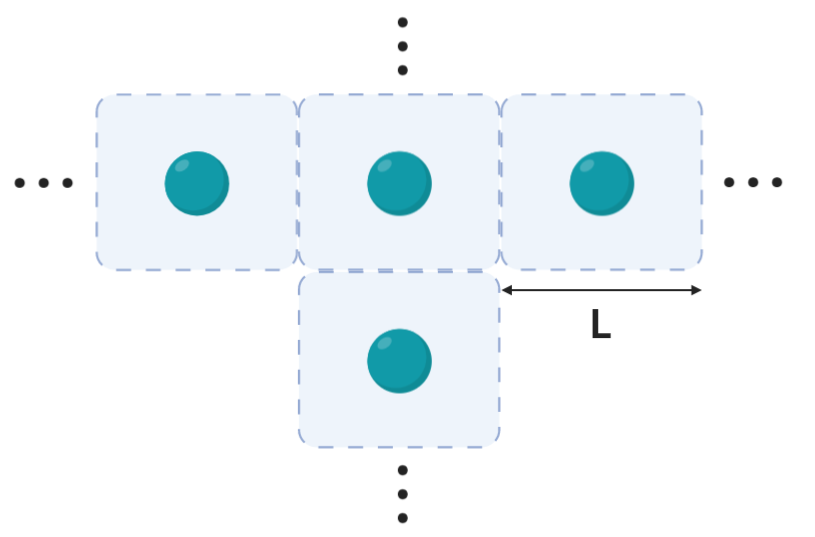
\includegraphics[scale = 0.55]{PBC.PNG}
	\caption{Centers of unit cells (blue) represent atoms or atomic clusters, as one would find in a periodic crystal. This structure is L-periodic. Here, only two dimensions have been shown, but crystals can exhibit periodicity in 3 dimensions as well (e.g. \ce{NaCl}). }
	\label{fig: Periodic Boundary Conditions}
\end{figure}

Here, $n_x, n_y, n_z$ are integers. We can thus consider solutions of the Schrodinger equation are satisfied by periodic plane wave states in the weak-binding approximation. In a region with volume $V$, these states can be written as:

\begin{align}
&\braket{\vec{r} | \vec{k}} = \frac{1}{\sqrt{V}}  \ e^{i\vec{k}\cdot\vec{r}} = \phi_{\vec{k}}(\vec{r})\\
&\int_V \phi_{\vec{k}}^{*}(\vec{r})\phi_{\vec{k}}(\vec{r})d\vec{r} = \braket{\vec{k}^{'} | \vec{k}} = \delta_{\vec{k}^{'} \vec{k}}
\end{align}  

Now we can consider linear combinations of these plane wave solutions as our wavefunction ansatz:

\begin{equation}
	\psi(\vec{r}) = \sum_{\vec{k}}c_{\vec{k}}\phi_{\vec{k}}(\vec{r})
\end{equation}

This can also be thought of as a Fourier series expansion of the wavefunction. In the continuum limit, we let $L \to \infty$, but keep $\psi(\vec{r})$ fixed. Mathematically, this means that the Fourier sum turns into a Fourier integral. 
\newline

We may now consider the volume in k-space per point in a unit cell (i.e. the atom/ cluster of atoms within a unit cell). Each point occupies a volume of $(2\pi/L)^3$ in k-space. For a 3D system, we can now define the \textbf{Density of States} (DOS) as:

\begin{equation}
D(E) = \frac{1}{V} \sum_k \delta(E-E_k)
\end{equation}

Here, $V$ is the volume occupied by the point in real space. In the continuum limit, this takes the form:

\begin{equation}
D(E) = \int \frac{d\vec{k}}{(2\pi)^3} \delta(E-E_k)
\end{equation}

This quantity tells us the number of states in a system at a particular energy $E$. The generalization of this quantity to N-dimensions is:

\begin{equation}
	D(E) = \int_{\mathbb{R^{N}}} \frac{d^N\vec{k}}{(2\pi)^N} \delta(E-E_k)
\end{equation}
 
We can also find the number of states with energy $\epsilon$ by computing:

\begin{equation}
	g(\epsilon) = \lim_{\Delta \epsilon \to 0}\int_{\epsilon}^{\epsilon + \Delta \epsilon} D(E)dE
\end{equation}

This is sometimes referred to as the \textit{Degree of Degeneracy}. Note that the regions where the DOS is zero can be understood as an energy bandgap.

\newpage
\subsection{Symmetries of the Hexagonal Lattice}

The symmetry points of the hexagonal lattice, some of which were used in the energy band diagrams in Section \ref{sec: DFT_simulations}, are shown below:

\begin{figure}[htb]
	\centering
	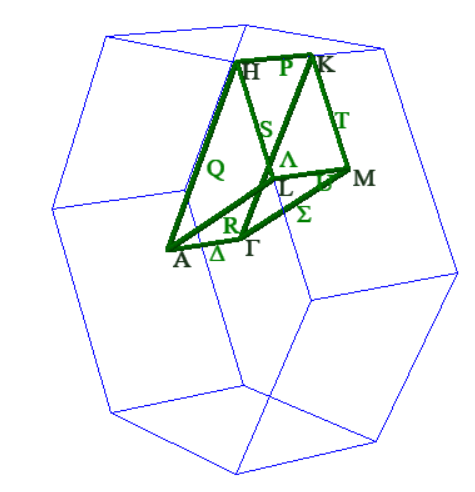
\includegraphics[scale = 0.7]{high_symmetry_points_hexagonal_lattice.PNG}
	\caption{High symmetry points and lines of the hexagonal lattice displayed within the first brillouin zone. Figure is from \cite{FBZ_symmetry_website}.}
	\label{fig: High_symmetry_points}
\end{figure}


\section{Tight-Binding Model}\label{sec: Tight Bonding}

The derivation and discussion in this section is based off of Chapter 9 of Kittel's \textit{Introduction to Solid State Physics} \cite{Kittel_SolidStatePhysics}. See the original paper by Slater et al. \cite{Original_Tight_Binding_Paper} or a theoretical review by Goringe et al. \cite{Tight_binding_theory_1997_Paper} for a more thorough discussion. 
\newline

The tight binding model is an approximate model used to calculate the electronic band structure using superpositions of wavefunctions for isolated atoms. This model is a one-electron model, but provides insight for calculations of surface states and several types of many-body problems and quasiparticle calculations. 
\newline

Consider an electron in its ground state $\phi(r)$ moving through a potential $U(r)$ of an isolated atom. Suppose that we can treat the influence of one atom on another to be small, we can write an approximate wavefunction for the electron as:

\begin{equation}
	\psi_k(r) = \sum_j C_{kj}\phi(r-r_j)
\end{equation}

Here, we sum over all lattice points. We also assumed that the primitive basis contains one atom. The function is of the Bloch form\footnotemark \ if $C_{kj} = N^{-1/2}e^{ik\cdot r}$, which gives the following wavefunction for a crystal of $N$ atoms:

\footnotetext{The wavefunction obeys the condition $\psi(r+T) = \exp(ik\cdot T)\psi_k(r)$, i.e. the wavefunction only varies by a phase factor upon translation.}

\begin{equation}
	\psi_k(r) = N^{-1/2}\sum_j e^{ik\cdot r} \phi(r-r_j)
\end{equation}

The first-order energy correction is then:

\begin{equation}
	\braket{k|H|k} = N^{-1} \sum_j \sum_k \exp[ik\cdot(r_j - r_m)] \braket{\phi_m | H | \phi_j}
\end{equation}

Here, $\braket{r|k} = \psi_k (r)$, and $\phi_m = \phi(r-r_m)$. Writing $\rho_m = r_m - r_j$, we get:

\begin{equation}\label{eq: Tight_binding_derivation_1}
	\braket{k|H|k} = \sum_m \exp[-ik\rho_m] \int dV \phi^{*}(r-\rho_m)H\phi(r)
\end{equation}

Neglecting all integrals in \ref{eq: Tight_binding_derivation_1} except those on the same atom or those between nearest neighbors connected by $\rho$, we can write:

\begin{equation}
	\int dV \phi^{*}(r)H\phi(r) = -\alpha ; \ \ \ \ \int dV \phi^{*}(r-\rho)H\phi(r) = -\gamma
\end{equation}

Assuming $\braket{k|k} = 1$, we have:

\begin{equation}\label{eq: tight_binding_hamiltonian_classical}
	\braket{k|H|k} = -\alpha -\gamma\sum_m \exp(-ik\cdot \rho_m) = \epsilon_k
\end{equation}

Hence, the energy of the electron in the tight-binding model can be written as:

\begin{align}
	E(k) \approx E_0 + \epsilon(k)
\end{align}

Where $E_0$ is the energy of the unperturbed single atom case. Note that this derivation is only valid for non-degenerate states; the derivation in the degenerate states case is slightly more involved.
\newline

In the second quantization formalism, the Hamiltonian takes the form:

\begin{equation}\label{eq: second_quant_tight_binding_hamiltonian}
	H = -t\sum_{<i,j>, \sigma} ( c_{i, \sigma}^{\dagger}c_{i, \sigma} + h.c.)
\end{equation}

\begin{itemize}
	\item $c_{i, \sigma}^{\dagger}, c_{i, \sigma}$ - creation and annihilation operators
	\item $\sigma$ - spin polarization
	\item $t$ - hopping integral
	\item $<i,j>$ - nearest neighbor index 
\end{itemize}

The hopping integral parameter in equation \ref{eq: second_quant_tight_binding_hamiltonian} corresponds to the transfer integral parameter $\gamma$ in equation \ref{eq: tight_binding_hamiltonian_classical}.


\section{DFT Notes}
These notes are based on Chapter 1 of \textit{Density Functional Theory: A Practical Introduction} \cite{DFT_A_Practical_Introduction}.
\subsection{Introduction}

Multi-electron Schrodinger equation:

\begin{equation}\label{Multi-electron SE}
\Big[-\frac{\hbar^2}{2m} \sum_{i=1}^{N}\nabla_{i}^2 + \sum_{i=1}^{N} V(r_i) + \sum_{i=1}^{N}\sum_{j<1} U(r_1, r_j) \Big ]\psi = E\psi
\end{equation}

Terms left to right: kinetic energy of electrons, interaction energy of electrons and atomic nuclei, interaction between different electrons. \newline

Hartree ansatz (decouple electronic wavefunctions):

\begin{equation}
\psi = \psi_1(r)\psi_2(r)\cdots\psi_N(r)
\end{equation}

Problem with solving the multi-electron SE (\ref{Multi-electron SE}) is that the dimensionality of the problem scales as 3N, with N being the number of electrons. For example, the \ce{C0_2} molecule wavefunction is a 66-dimensional function; a nanocluster of 100 Platinum atoms would require $\sim$23,000 dimensions! Hence, more efficient techniques are required to solve large multi-body problems. 
\newline

Define the density of electrons at a particular position in space, r:

\begin{equation}
n(r) = 2\sum_{i} \psi_{i}^{*}(r)\psi_{i}(r)
\end{equation}

This summation goes over all the individual electron wavefunctions. The factor of 2 arises from the Pauli exclusion principle.


\subsection{Hohenberg-Kohn Theorems}

\begin{itemize}
	\item \textit{Theorem 1}:
	The ground-state energy from the Schrodinger equation is a unique functional of the electron density:
	\begin{equation}
	E = E[n(r)]
	\end{equation}
	
	\item \textit{Theorem 2}:
	The electron density n(r) that minimizes the overall functional is the true electron density corresponding to the full solution of the Schrodinger equation.
\end{itemize}

This is an important result because it effectively reduces the 3N-dimensional problem to a 3-dimensional problem.
\newline

The energy functional can be written as:

\begin{equation}
E[{\psi_i}] = E_{known}[{\psi_i}] + E_{XC}[{\psi_i}]
\end{equation}

Here the functional is split into the analytic form, $E_{known}[{\psi_i}] $, and 'everything else", in the exchange-correlation energy $E_{XC}[{\psi_i}]$. The known form of the energy functional has four terms:

\begin{equation}
E_{known}[{\psi_i}] = \frac{\hbar^2}{2m}\sum_{i}\int\psi_{i}^{*}\nabla^2\psi_{i}d^3r + \int V(r)n(r)d^3r +\frac{e^2}{2}\int\int\frac{n(r)n(r')}{|r-r'|}d^3rd^3r' + E_{ion}
\end{equation}

Terms in order: electron kinetic energies, Coulomb interaction between electrons and the nuclei, Coulomb interaction between pairs of electrons, Coulomb interaction between pairs of nuclei. The $E_{XC}[{\psi_i}]$ term is known as the exchange-correlation functional, which is included to capture all of the quantum-mechanical effects that are not included in the above terms.

\subsection{Kohn-Sham Scheme}
Kohn and Sham showed that the correct electron density n(r) can be found by solving a set of single-electron equations:

\begin{equation}\label{Kohn_Sham scheme}
\Big[ \frac{\hbar^2}{2m}\nabla^2 + V(r) + V_H(r) + V_{XC}(r) \Big] \psi_{i}(r) = \epsilon_{i}\psi_{i}(r)
\end{equation}

The V(r) potential defines the interaction between an electron and a collection of atomic nuclei. The Hartree potential, $V_{H}(r)$ is defined by:

\begin{equation}
V_{H}(r) = e^2 \int\frac{n(r')}{|r-r'|}d^3r'
\end{equation}

This potential describes the Coulomb repulsion between the electron being considered in one of the Kohn-Sham equations (\ref{Kohn_Sham scheme}) and the total electron density of all electrons in the problem. This potential also includes a self-interaction contribution because the electron being considered is also part of the total electron density, so part of $V_H$ involves a Coulomb interaction between an electron and itself. This is in reality an unphysical interaction, however it is accounted for in the $V_{XC}$ potential. $V_{XC}$ corrects for several such effects; it defines the exchange and correlation contributions to the single electron equations. We can define this potential as a functional derivative \footnote{Not quite identical mathematically to a regular derivative.} of the exchange-correlation energy seen before:

\begin{equation}
V_{XC}(r) = \frac{\delta E_{XC}(r)}{\delta n(r)}
\end{equation}

It may seem that this scheme provides a circular argument: To solve the Kohn-Sham equations, we need the Hartree potential $V_H$, and to get $V_H$ we need n(r), and to get n(r) we need the single electron wavefunctions, but to get the single electron wavefunctions we need to solve the Kohn-Sham equations! This problem is treated by following an iterative process (one suitable by computational means, say):
\begin{enumerate}
	\item Define a trial electron density n(r)
	\item Solve the Kohn-Sham equations using this trial n(r) to find the single-electron wavefunctions, $\psi_{i}(r)$
	\item Calculate the electron density from the wavefunctions obtained in part (2) as: $n_{KS}(r) = 2\sum_{i}\psi_{i}^{*}(r)\psi_{i}(r)$
	\item Compare $n_{KS}(r)$ to the trial n(r). If the two densities are sufficiently close, then this is the ground-state electron density, and can be used to compute the total energy. If the densities are different, then we must update the trial n(r) somehow and proceed from step 2 again.
\end{enumerate}

It is evident that this system is self-consistent.


\subsection{Exchange-Correlation Functional}

The true form of the exchange-correlation functional whose existence is guaranteed by the HK-Theorem is simply not known. In one case, this functional can be derived exactly: the uniform electron gas. Here, the electron density is constant over all space, i.e. $n(r)$ = constant. We set the exchange-correlation potential at each position to be the known exchange-correlation potential from the uniform electron has at the electron density observed at that position:

\begin{equation}
V_{XC}(r) = V_{XC}^{electron \ gas}[n(r)]
\end{equation}

In this approximation we used only the local density to define the approximate exchange-correlation functional, so it is called the \textit{local density approximation} (LDA). While the LDA approximation allows us to completely define the Kohn-Sham equations, it does not solve the true Schrodinger equation because we are not using the true exchange-correlation functional.
\newline

There exists another class of approximate functionals, called the \textit{Generalized Gradient Approximation} (GGA). This approximation uses information about the local electron density and local gradient in the electron density. It remains a challenge to find the form of the exchange-correlation functional that truly resembles nature, and is an active area of research.



\newpage
\nocite{*}
\printbibliography[heading=bibintoc, title={References}]



\end{document}